%!TEX root = ../risk_report.tex

\chapter{Findings} \label{chap:findings}

    Findings are organised according to the formulation of areas of interest as questions. These questions progress from general frequency counting (Q1), through experiential meanings (Qs 2--7), to risk as modifier (Qs 8 \& 9) and finally to arguability (Q10). Discussion of the general significance of individual findings is also presented in this section, as the Discussion section synergises all findings to explain the discourse-semantics of risk.

    \vspace{5mm}
    \noindent\begin{tcolorbox}[colback=yellow!5,colframe=yellow!40!black,title=Summary: an example]
    \parbox{1\textwidth}{%
    Summaries of each major finding will be presented in highlighted text boxes.}
    \end{tcolorbox}
    \vspace{5mm}

    \noindent An \emph{IPython Notebook} interface for navigating the corpus \cite<see>{mckinney_python_2012}, as well as the code used to interrogate it and the findings we produced, are available online, at \url{https://github.com/interrogator/corpkit} and \url{https://github.com/interrogator/risk}. A non-interactive version is available at \url{http://nbviewer.ipython.org/github/interrogator/risk/blob/master/risk.ipynb}. This Notebook does not suffer from spatial limitations, and thus contains additional information, including the exact Tregex queries used in interrogations, as well as complete lists of the concordance lines discussed only briefly here. Tools and results from other kinds of corpus linguistic analysis, such as keywording and collocation, are also available there, but have not been described here.

\section{How frequently do risk words appear?} \FloatBarrier

    %We successfully located a number of lexicogrammatical sites of change within clauses containing a risk word. 

    The first point of interest was the overall frequency of risk words in the NYT (Figure \ref{fig:relative_frequency_of_risk_words}) and the distribution of risk words by word class (nominal, verbal, adjectival\slash adverbial), absent any consideration of surrounding grammar (see Figure \ref{fig:wordclasses}). In terms of the relative frequency of risk words, we note a general upward trend, with a number of peaks and troughs worthy of further investigation. In terms of word classes of risk, we found that not only are nominal forms by far the most common in the NYT, but that it is nominal risk words that vary the most in frequency, with the other categories remaining more or less stable. Interestingly, in the span for which we have no data (1964--1986), adjectival forms overtake verbal forms of risk in frequency.

    %Using our reference corpus, we checked to see whether nominals were becoming more frequent within the NYT more generally.

    \noindent
    \begin{figure}[htb!]
    \centering
    \begin{minipage}{.45\textwidth}
    \centering
    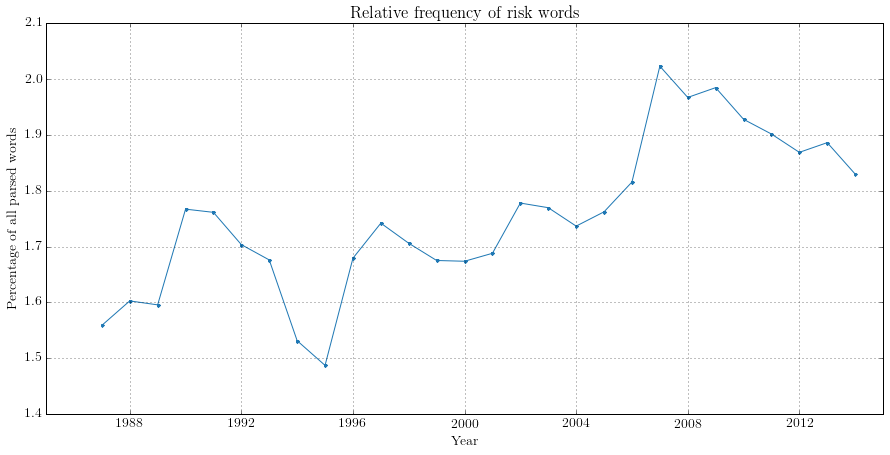
\includegraphics[width=.95\textwidth]{../images/relative_frequency_of_risk_words.png}
    \caption{Relative frequency of risk words}
    \label{fig:relative_frequency_of_risk_words}
    \end{minipage}%
    \begin{minipage}{.55\textwidth}
    \centering
    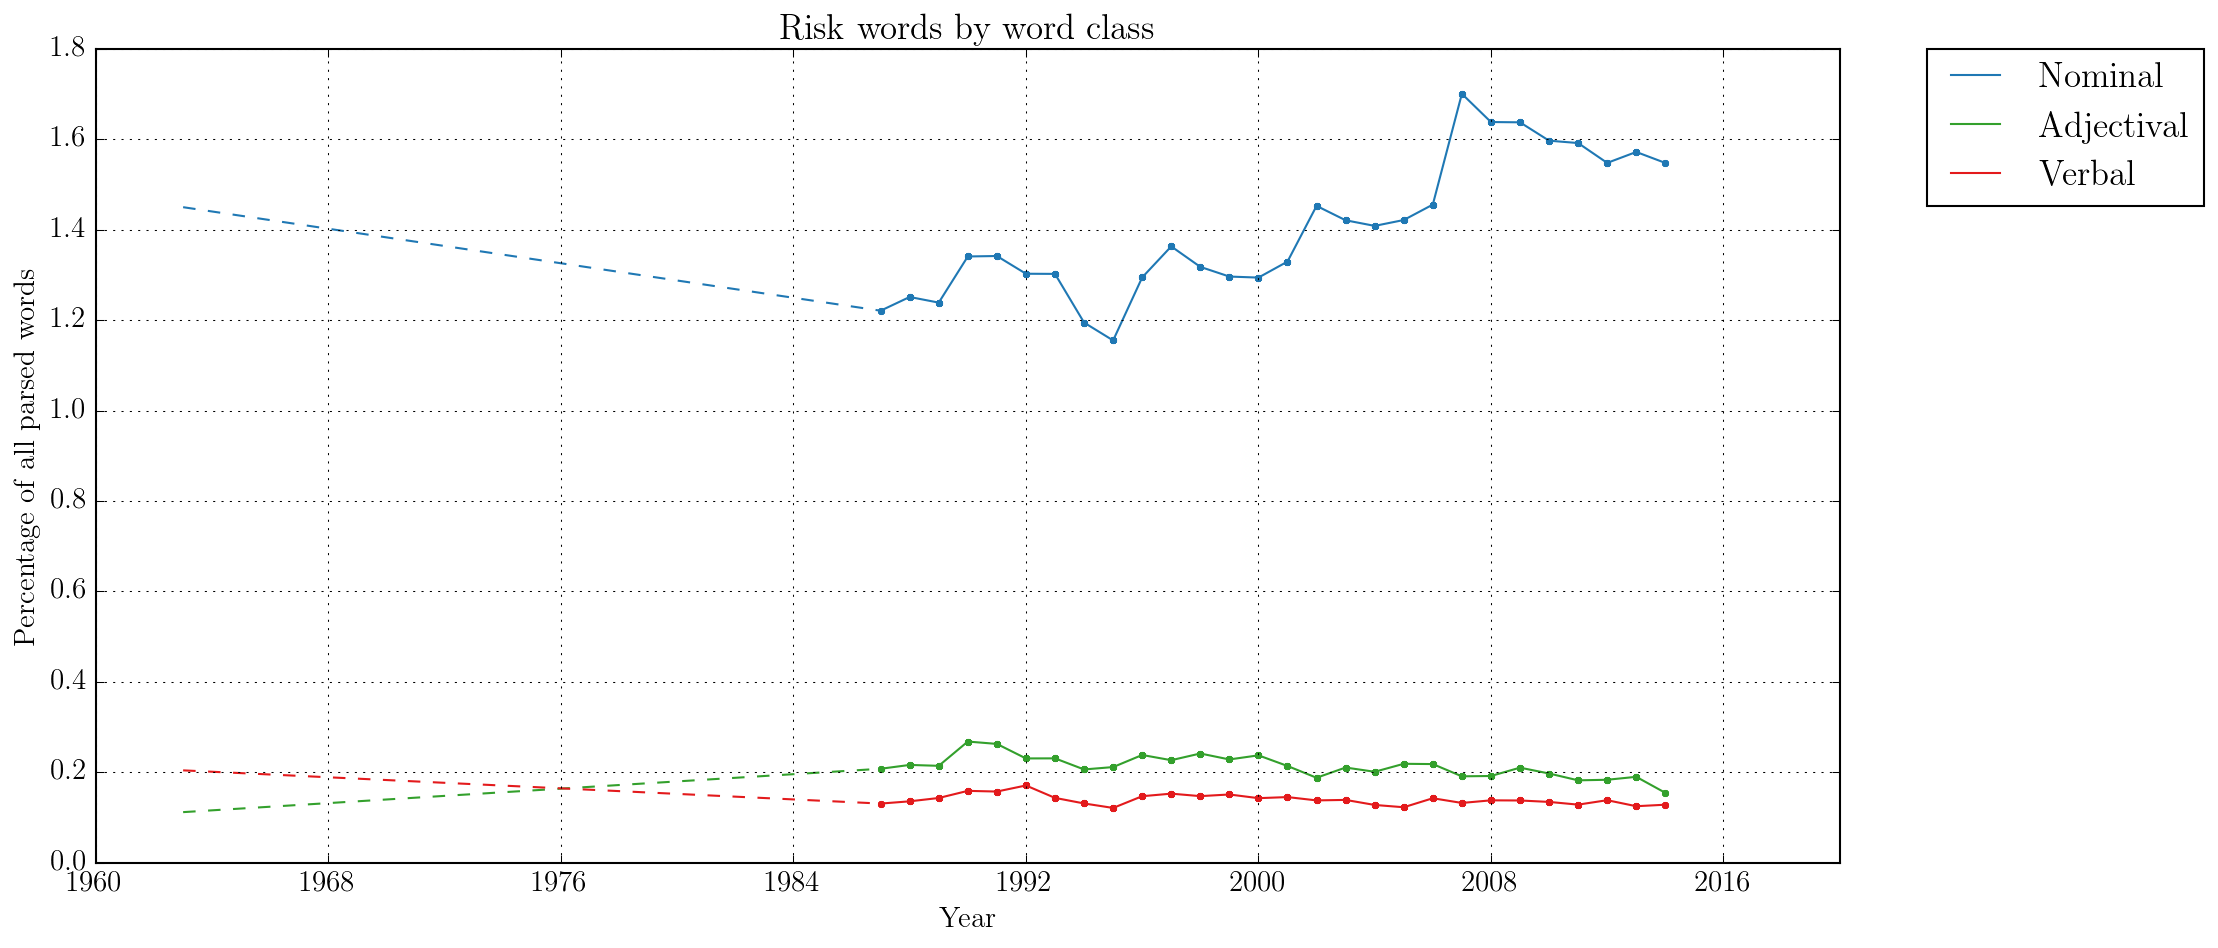
\includegraphics[width=.95\textwidth]{../images/risk_words_by_word_class.png}
    \caption{Relative frequency by word class}
    \label{fig:wordclasses}
    \end{minipage}
    \end{figure}

    \begin{figure}[htb!]
    \centering
    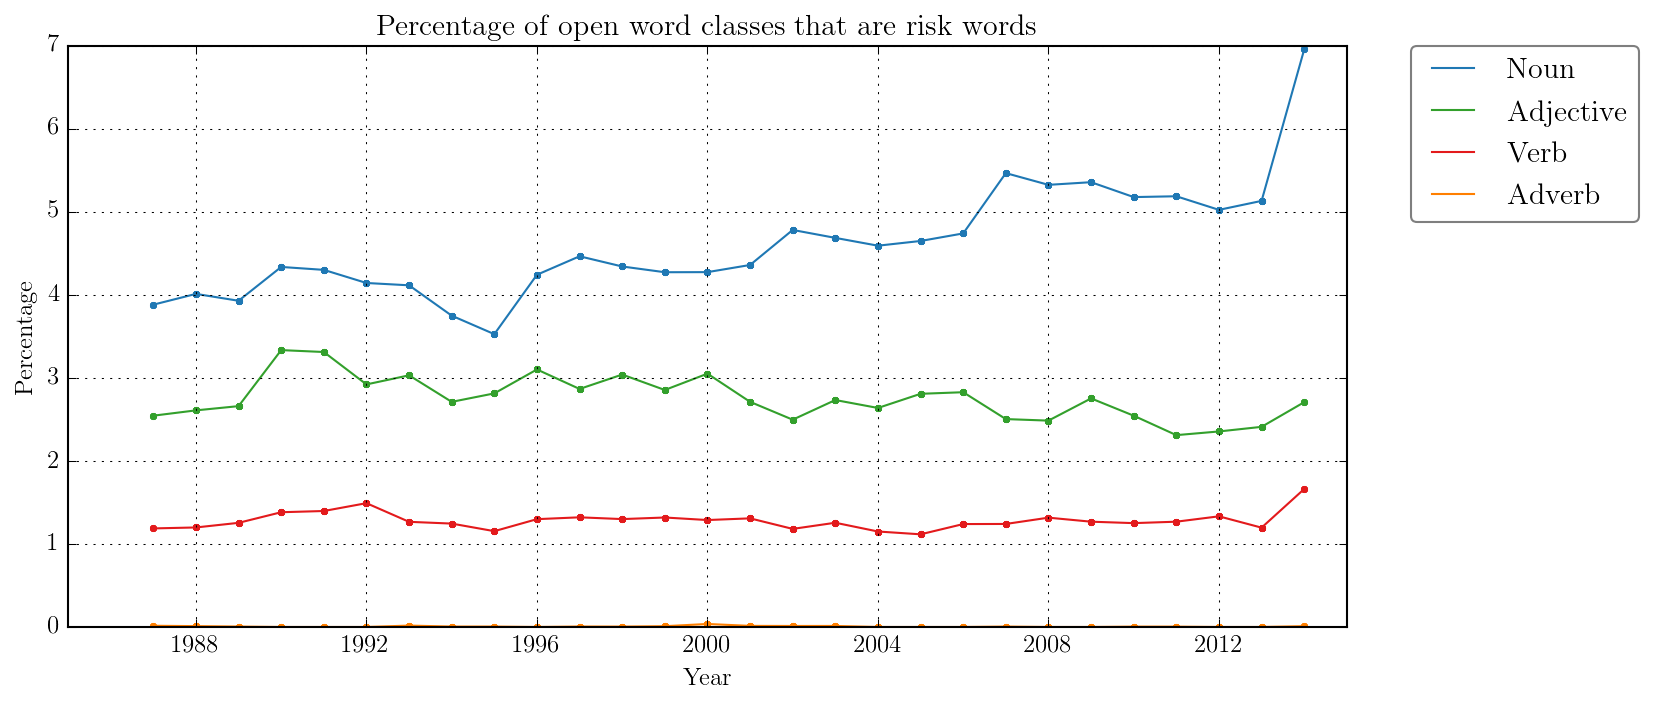
\includegraphics[width=0.7\textwidth]{../images/percentage-of-open-word-classes-that-are-risk-words.png}
    \caption{Percentage of each open word class that are risk words}
    \label{fig:eachperc}
    \end{figure}



    %\begin{figure}[htb!]
    %\centering
    %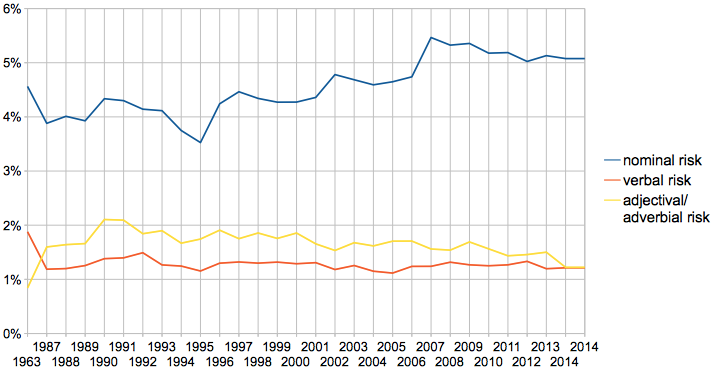
\includegraphics[width=0.75\textwidth]{../images/relwordclass.png}
    %\caption{Risk words by word class as percentage of all parsed words}
    %\label{fig:relwordclass}
    %\end{figure}

    We compared this against the relative frequencies of nominal, verbal and adjectival\slash adverbial lexical items in the corpus as a whole, in order to account for any trends toward nominalisation in our dataset more generally (Figure \ref{fig:wordclasses}). This showed that even when compared to potential trends toward nominalisation generally (Figure \ref{fig:eachperc}), nominal risks are becoming more frequent in later NYT editions. 

    This is an important preliminary finding: verbal groups form the nucleus of experiential meanings, the shift toward nominal risk is in effect a shift toward risk discourse where risk is not the central event being depicted, but is instead a player within a broader range of events. Furthermore, given that nominal risk is closer to synonymous with harm or threat, shifts toward nominal risks are indeed evidence for Lupton's argument that the semantics of risk increasingly reflect negative outcomes.

    %As nouns congruently perform the role of Participant, the shift toward nominal risks is related to the `participantification' of risk discussed in Section \ref{sect:exprole}.

    These initial findings guided the rest of the investigation: particular attention was paid to nominal risks, as these were the site of the most longitudinal change. That said, these categories provide merely a categorisation of the formal features of risk words. Functionally, things are substantially more complicated: \emph{running a risk}, for example, while featuring a nominal risk, is in reality a risk process; similarly, though risk is nominal in \emph{risk management}, it functions as a modifier, rather than a participant. Accordingly, in our analysis, functional categories are typically preferred over formal categories where possible.

    A similar question is the number of unique risk words appearing per year. Figure \ref{fig:diffriskwords} demonstrates that there is a general increase in the relative number of unique risk words over time.\endnote{1963 is excluded from analysis here, as poor quality OCR created a number of non-word results such as \emph{risks-wnrk}, \emph{risks.North} and \emph{risks.With}.}

    \begin{figure}[htb!]
    \centering
    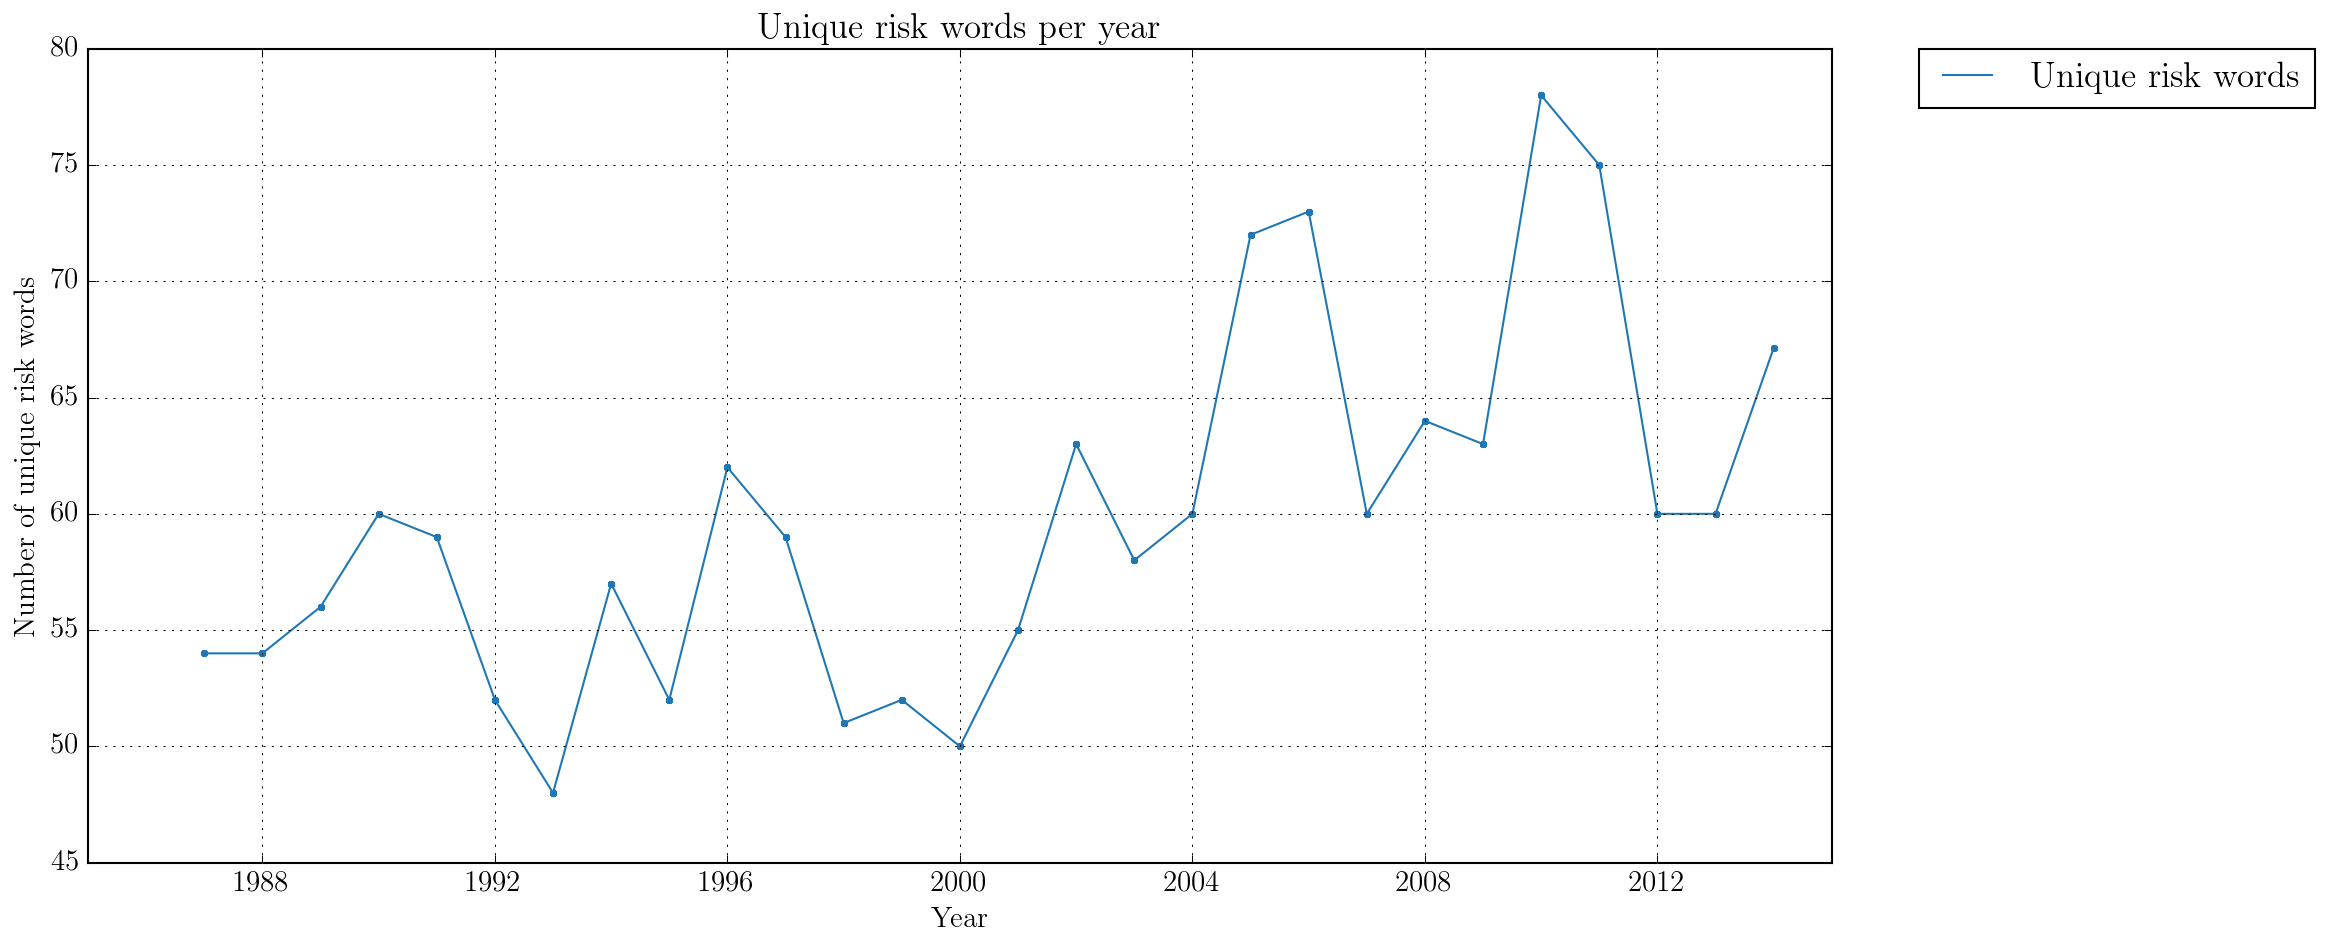
\includegraphics[width=0.7\textwidth]{../images/unique_risk_words_per_year.png}
    \caption{Unique risk words}
    \label{fig:diffriskwords}
    \end{figure}

    \vspace{5mm}\noindent\begin{tcolorbox}[colback=yellow!5,colframe=yellow!40!black,title=Summary: frequency of risk words]
    \parbox{1\textwidth}{%
    Risk words appear to be increasing in relative frequency, with modest increases in the number of unique risk words per year.}
    \end{tcolorbox}
    \vspace{5mm}

\section{Which experiential roles do risk words occupy?} \label{sect:exprole} \FloatBarrier

    In a systemic-functional conceptualisation of the experiential metafunction of language (that is, the ways in which language is used to communicate who did what to whom), risk words may take the form of a Participant (\emph{The risk was there}), Process (\emph{I risked it}) or a Modifier (\emph{a risky encounter}). Though these pattern to some extent with word classes (e.g. \emph{participant = noun, process = verb, modifier = adjective}), word classes on the whole are a poor indication of functional role, especially in genres such as print news journalism,  which rely heavily on nominalisation and grammatical metaphor to pack large amounts of experiential information into each clause. As shown in Table \ref{tab:class_and_role}, for example, nominal risks commonly perform Modifier functions, and adjectival functions often perform Participant functions.

    \begin{table}
    \small
    \centering
    \begin{tabular}{|l|l|l|}
    \hline
    \textbf{Example}       & \textbf{Word class}     & \textbf{Experiential role}     \\ \hline
    \emph{It was risky}  & Adjective  &  Participant   \\ \hline
    \emph{A risking of lives} & Noun  &  Nominalised process   \\ \hline
    \emph{Risk management}  & Noun & Modifier   \\ \hline
    \end{tabular}
    \caption{Key differences between word class and experiential role}
    \label{tab:class_and_role}
    \end{table}

    Using Stanford CoreNLP's dependency parses, we counted the frequency of risk words within these three functional roles (Figure \ref{fig:funcrole}). In line with the results from word-class based searching, we find that risk as a Process is declining in use. Risk as Modifier, patterning in part with adjectival risk, appears to be increasing. That said, we can also see here the affordances of a functional grammar in corpus assisted discourse research: in this case, much richer evidence of changing usage of risk can be found through an understanding of its semantic function rather than its word class alone.

    The decline of risk as a Process can be read as a shift away from the `risk frame' identified by \citeA{fillmore_toward_1992}. Their frame is essentially a mapping of the possible kinds of participants that can occur when risk is used as a process. In a very typical risk process, such as \emph{He risked everything}, \emph{He} is the Actor and everything is the \emph{Valued Object}. Risk as participant is less likely to explicitly index the major components of the risk frame: in \emph{The risk must be weighed against the benefit}, we are not given any specific information about the configuration of the risk scenario. (Risk as modifier encompasses a number of functional roles. As such, we leave this discussion for sections \ref{sect:mod_one} and \ref{sect:mod_two}.)

    Like with our analysis of the word classes of risk, we can also understand the shifts in the experiential roles of risk words as evidence for an increasing implicitness of risk in NYT news discourse. As mentioned earlier, in a systemic-functional conceptualisation of language, the process is the locus of experiential meaning---it selects the kinds of participants that can occur as its arguments. Modifiers and circumstances are the least consequential kinds of experiential meaning, as they provide ancillary or supplementary kinds of meaning, regarding the manners in which processes were performed, or characteristics of participants. 

    %Nominalisation is also closely tied to arguability. This link is discussed in Section \ref{sect:arguability}.

    %``From studies comparing identical and fraternal twins, it is estimated that genetic factors account for 40 to 60 percent of the variation in the risk for addiction.''

    %That was just one day after Richard S. Fuld Jr. , Lehman 's chief executive , announced a new strategy that he said would `` accomplish a significant de-risking of our balance sheet , '' in part by putting risky assets into a new company it would spin off to shareholders next year .

    % `` Ambac has consistently emphasized that in this period of extreme uncertainty in the capital markets , the de-risking and de-leveraging of our balance sheet is our highest priority , '' David W. Wallis , the chief executive , said in a news release .

    \begin{figure}[htb!]
    \centering
    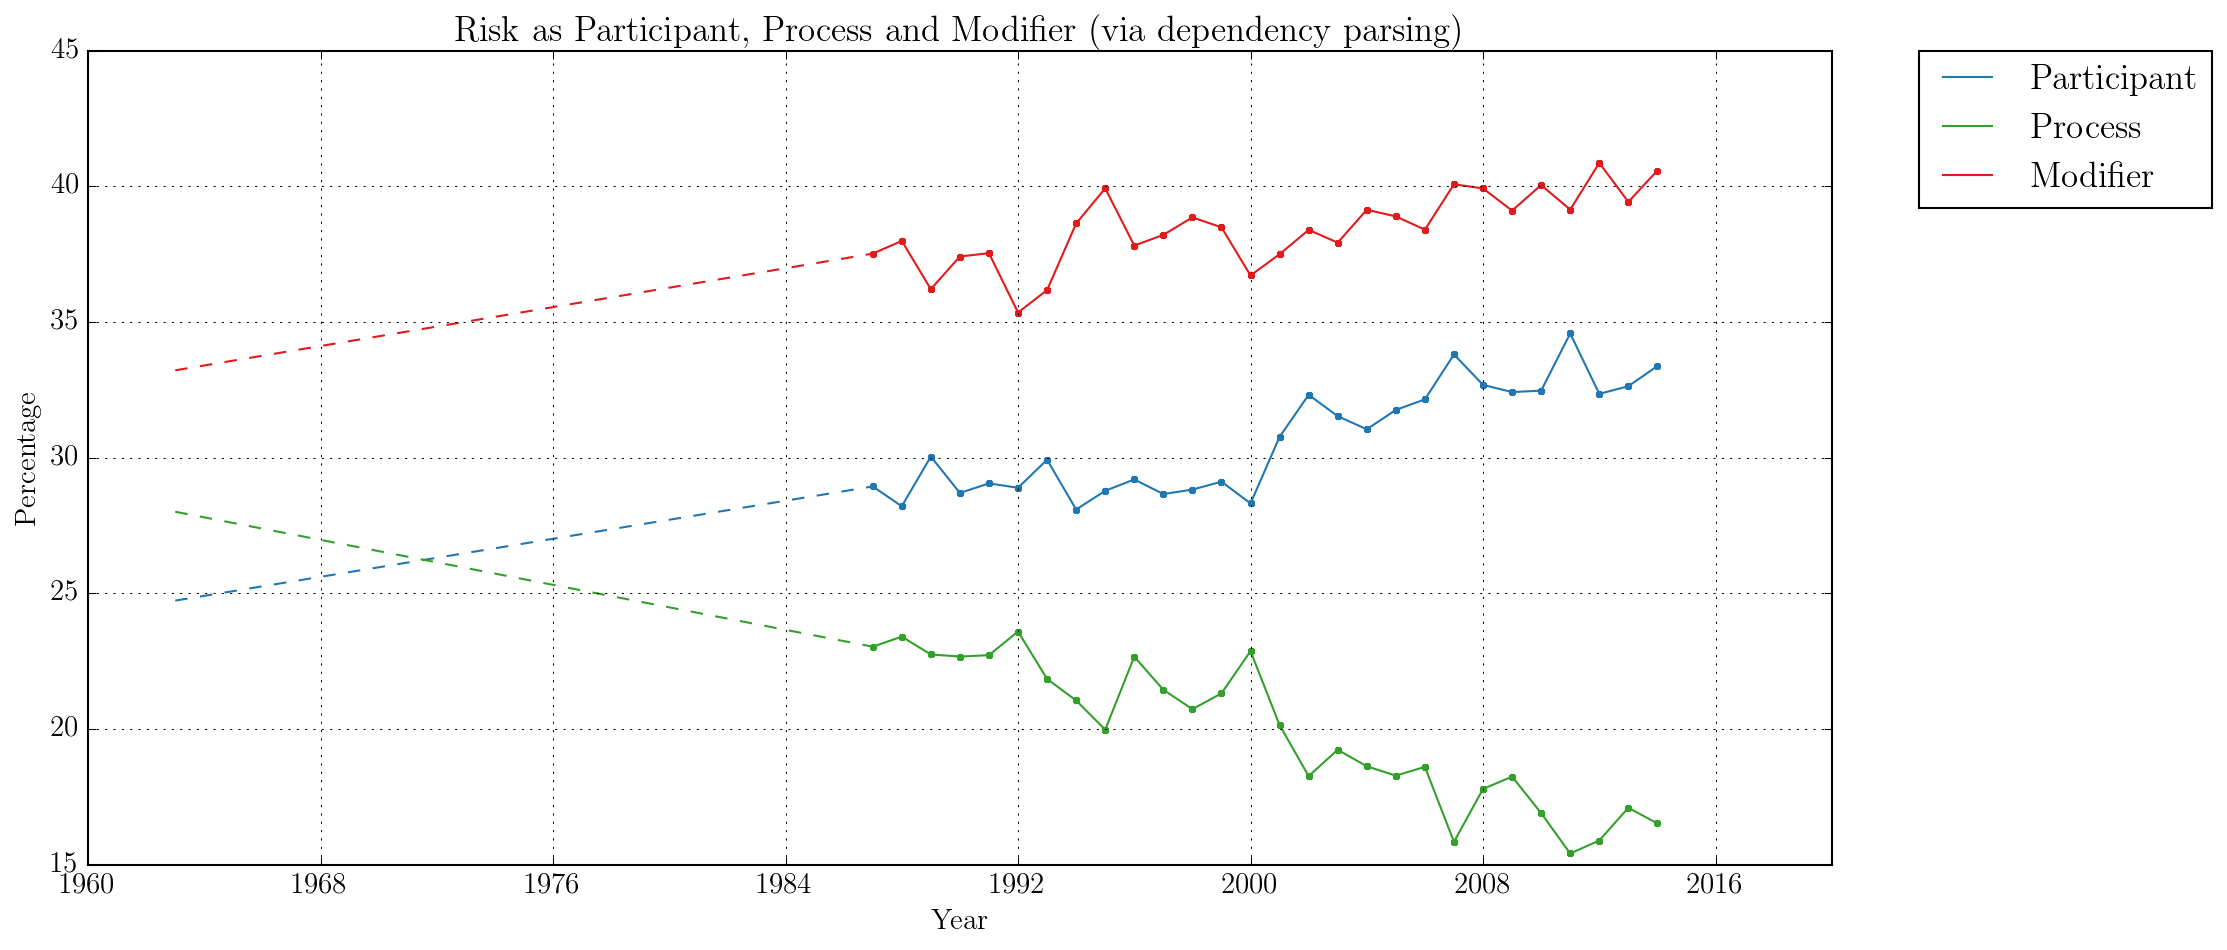
\includegraphics[width=0.7\textwidth]{../images/risk-as-participant-process-and-modifier-via-dependency-parsing.png}
    \caption{Experiential roles of risk words}
    \label{fig:funcrole}
    \end{figure}

    %~\ \todo[inline,color=yellow!40]{\noindent More discussion here, perhaps, as well as the above chart as relative frequencies. I may also have to account for risk within prepositional phrases here.}
    
    %only when the risk word forms the head of these groups, rather than a dependent/modifier (e.g. \emph{a risky decision}).

    \vspace{5mm}\noindent\begin{tcolorbox}[colback=yellow!5,colframe=yellow!40!black,title=Summary: experiential function of risk words]
    \parbox{1\textwidth}{%
    Risk as a process is declining in use, and has been overtaken in frequency by risk as a participant.}
    \end{tcolorbox}
    \vspace{5mm}

\section{Is risk more commonly in the position of experiential subject or experiential object?} \FloatBarrier

    Risk as a participant may take the form of an experiential subject or an experiential object.\endnote{These are not particularly meaningful distinctions in SFL, as the role of participants depends on the process type. Though process type identification is becoming more and more feasible \cite<see>{odonnell_uam_2008}, at the time of our investigation, we lacked resources to automatically distinguish between process types, and thus relied on borrowed notions of experiential subject- and objecthood.} 
    Our first area of interest was the proportion of each, with respect to general trends in the NYT. As shown in Figure \ref{fig:bestexpsubjobj}, risk is more commonly an object than a subject. It is also apparent that risk as experiential subject is on an static trajectory, while risk as experiential object is inbound. The significance of this is discussed in more depth in Section \ref{sect:arguability}.

    \begin{figure}[htb!]
    \centering
    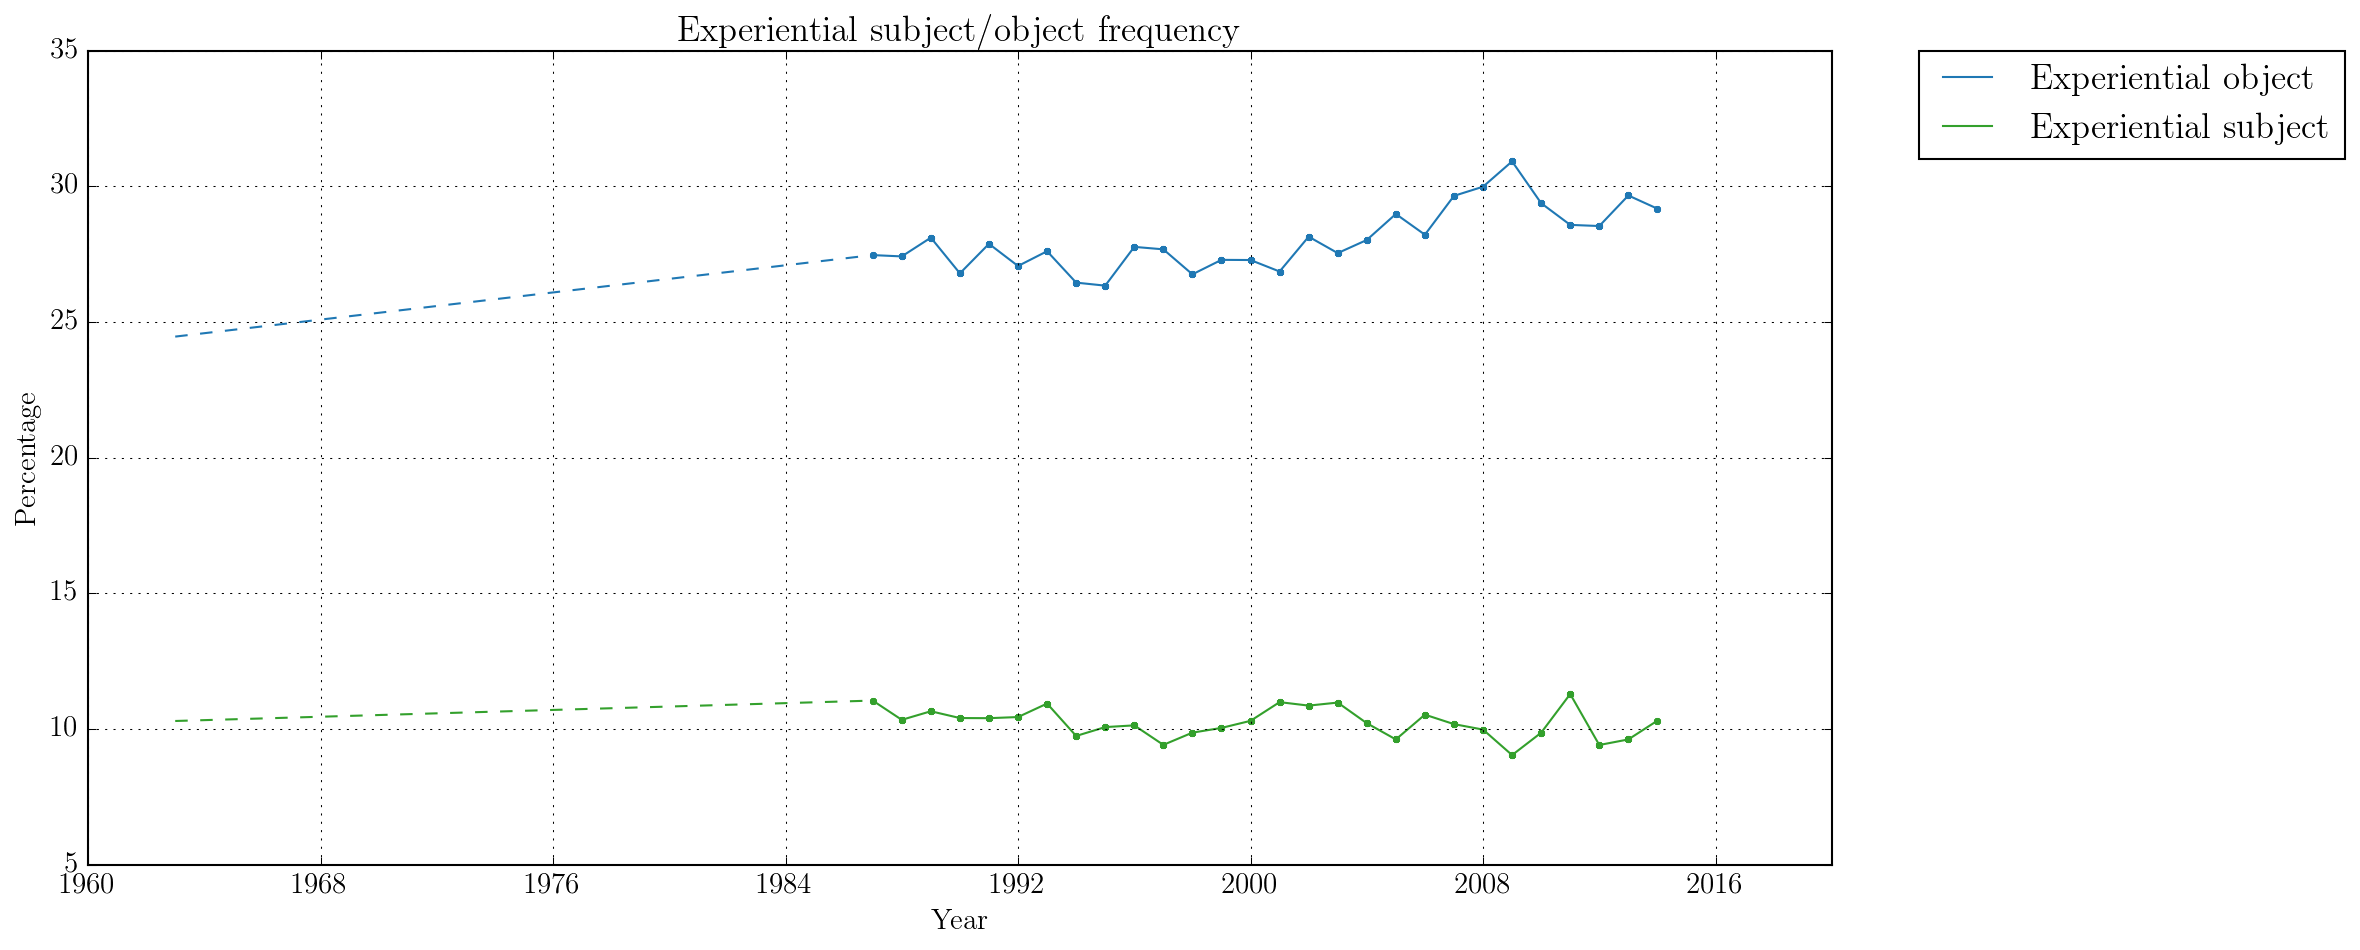
\includegraphics[width=0.75\textwidth]{../images/experiential_subject_object_frequency.png}
    \caption{Risk as experiential subject and object as percentage of all risk roles}
    \label{fig:bestexpsubjobj}
    \end{figure}
    %

    \begin{table}[tb]\footnotesize
    \centering
    \addvbuffer[12pt 8pt]{\begin{tabularx}{0.75\textwidth}{|X|X|}
    \hline
    \textbf{As subject} & \textbf{As object} \\ \hline
    \textit{But the most prevalent \textbf{risk} for the average traveler to Peru is the high altitude of the Andes}   & \textit{The company has resolved accounting problems, he said, and stabilized profit margins, while new management has reduced the company's \textbf{risks}}  \\ \hline
    \textit{The \textbf{risk} would be that the stock would recover during the period that the investor was out of the stock}   & \textit{But an empty village is a big \textbf{risk}.}  \\ \hline
    \textit{But the \textbf{risk}, though very small, that a man facing execution could win a new trial raises the question why this rule has proved so hard to follow}   & \textit{They said there was only a little \textbf{risk}, and now he 's not with us anymore} \\ \hline
    \end{tabularx}}
    \caption{Examples of risk as experiential subject and object in 2001}
    \label{tab:subj_conc}
    \end{table}

    \vspace{5mm}\noindent\begin{tcolorbox}[colback=yellow!5,colframe=yellow!40!black,title=Summary: risk as experiential subject\slash object]
    \parbox{1\textwidth}{%
    Risk is more often an experiential object than an experiential subject. The gap has widened considerably over time.}
    \end{tcolorbox}
    \vspace{5mm}

\section{What processes are involved when risk is a participant?} \FloatBarrier

    We then wanted to determine the most common processes in which risk as a participant is involved. Tables \ref{tab:subj} and \ref{tab:obj} show the top twenty processes for risk as experiential subject and object, taking passivisation into account.\endnote{\emph{Take} and \emph{run} are removed from the object column here, as \emph{take risk} and \emph{run risk} are considered risk processes.}~

    % this below doesn't count agent as an experiential subject, and it should! also copula

    \begin{table}[htb!]
    \centering
    \addvbuffer[12pt 8pt]{\begin{minipage}{.35\textwidth}
    \small
    \begin{tabularx}{1.0\textwidth}{|>{\raggedright}X|l|}
    \hline
    \textbf{Processes when risk is experiential subject} & \textbf{Total} \\ \hline
    be                                      & 8954  \\ \hline
    increase                                & 460   \\ \hline
    outweigh                                & 278   \\ \hline
    rise                                    & 269   \\ \hline
    say                                     & 222   \\ \hline
    come                                    & 201   \\ \hline
    remain                                  & 192   \\ \hline
    go                                      & 190   \\ \hline
    have                                    & 179   \\ \hline
    make                                    & 148   \\ \hline
    seem                                    & 148   \\ \hline
    involve                                 & 145   \\ \hline
    grow                                    & 133   \\ \hline
    exist                                   & 127   \\ \hline
    take                                    & 121   \\ \hline
    become                                  & 120   \\ \hline
    lose                                    & 120   \\ \hline
    include                                 & 113   \\ \hline
    appear                                  & 111   \\ \hline
    pay                                  & 100   \\ \hline
    \end{tabularx}
    \caption{Processes when risk is \mbox{experiential} subject}
    \label{tab:subj}
    \end{minipage}} \hspace{1cm} % This must go next to `\end{minipage}`
    \addvbuffer[12pt 8pt]{\begin{minipage}{.35\textwidth}
    \small
    \begin{tabularx}{1.0\textwidth}{|>{\raggedright}X|l|}
    \hline
    \textbf{Processes when risk is experiential object} & \textbf{Total} \\ \hline
    %take                                             & 11459 \\ \hline
    reduce                                           & 5609  \\ \hline
    pose                                             & 4179  \\ \hline
    increase                                         & 4063  \\ \hline
    %run                                              & 3506  \\ \hline
    have                                             & 2879  \\ \hline
    carry                                            & 2115  \\ \hline
    face                                             & 1477  \\ \hline
    raise                                            & 1115  \\ \hline
    minimize                                         & 1009  \\ \hline
    assess                                           & 841   \\ \hline
    create                                           & 731   \\ \hline
    outweigh                                         & 704   \\ \hline
    avoid                                            & 683   \\ \hline
    present                                          & 619   \\ \hline
    assume                                           & 593   \\ \hline
    consider                                         & 588   \\ \hline
    see                                              & 563   \\ \hline
    understand                                       & 493   \\ \hline
    accept                                           & 492   \\ \hline
    weigh                                        & 473   \\ \hline
    eliminate                                        & 450   \\ \hline
    
    \end{tabularx}
    \caption{Processes when risk is experiential object}
    \label{tab:obj}
    \end{minipage}}
    \end{table}

    Interesting here is the dominance of processes seeking to quantify risk. Also salient is the presence of a large set of mental processes (\emph{seem, appear, assess, understand, accept}). This may be seen as evidence for an increased demand for the control of risk (see discussion in sections \ref{sect:mod_two}; contrast with section \ref{sect:highpotential})).

    %Future research is planned to divide processes with risk participants into the systemic functional conceptualisation of process types. Potentially, we could determine whether or not risks are shifting to or from mental to material.

    \vspace{5mm}\noindent\begin{tcolorbox}[colback=yellow!5,colframe=yellow!40!black,title=Summary: processes with risk participants]
    \parbox{1\textwidth}{%
    When risk is a participant, quantification is often at the centre of the experiential meaning. The high proportion of mental processes highlights a portrayal of risks as perceived.}
    \end{tcolorbox}
    \vspace{5mm}

\section{How are participant risks modified?} \label{sect:highpotential} \FloatBarrier

    Most commonly, risk as a participant is modified through adjectival pre-head modification or post-head modification with a subordinate clause or prepositional phrase. Ignoring the distinction between subject and object risk, and collapsing pre-head and post-head kinds of modification, Tables \ref{tab:prehead} and \ref{tab:posthead} show the most common pre- and post-head modifiers of risk as a participant.

    \begin{table}%[htb!]
    \centering
    \addvbuffer[12pt 8pt]{\begin{minipage}{0.35\textwidth}
    \raggedleft
    \small
    \begin{tabular}{|l|l|}
    \hline
    \textbf{Pre-head modifier}     & \textbf{Total} \\ \hline
    high         & 4753  \\ \hline
    great        & 3444  \\ \hline
    big          & 1672  \\ \hline
    political    & 1520  \\ \hline
    potential    & 1340  \\ \hline
    financial    & 1164  \\ \hline
    low          & 1056  \\ \hline
    more         & 1051  \\ \hline
    significant  & 1003  \\ \hline
    serious      & 935   \\ \hline
    real         & 869   \\ \hline
    little       & 761   \\ \hline
    own          & 713   \\ \hline
    substantial  & 547   \\ \hline
    less         & 541   \\ \hline
    such         & 514   \\ \hline
    calculated   & 469   \\ \hline
    considerable & 463   \\ \hline
    possible     & 458   \\ \hline
    other        & 423   \\ \hline
    \end{tabular}
    \caption{Pre-head modification of participant risk}
    \label{tab:prehead}
    \end{minipage}} \hspace{1cm}% This must go next to `\end{minipage}`
    \addvbuffer[12pt 8pt]{\begin{minipage}{0.35\textwidth}
    \raggedright
    \small
    \begin{tabular}{|l|l|}
    \hline
    \textbf{Post-head modifier} & \textbf{Total} \\ \hline
    cancer             & 2344  \\ \hline
    disease            & 1777  \\ \hline
    attack             & 1597  \\ \hline
    death              & 1025  \\ \hline
    injury             & 823   \\ \hline
    infection          & 811   \\ \hline
    loss               & 408   \\ \hline
    war                & 391   \\ \hline
    failure            & 383   \\ \hline
    inflation          & 368   \\ \hline
    problem            & 346   \\ \hline
    default            & 336   \\ \hline
    stroke             & 325   \\ \hline
    complication       & 288   \\ \hline
    damage             & 251   \\ \hline
    transmission       & 248   \\ \hline
    harm               & 244   \\ \hline
    aid                & 227   \\ \hline
    recession          & 217   \\ \hline
    accident           & 208   \\ \hline
    \end{tabular}
    \caption{Pre-head modification of participant risk}
    \label{tab:posthead}
    \end{minipage}}
    \end{table}

    Some of these modifiers are undergoing longitudinal trajectory change. As can be seen in Figure \ref{fig:reladjrisk}, \emph{calculated risk} has an outbound trajectory, decreasing steadily. The large number of occurrences projected for 1963, however, is partially the result of the 1962 Broadway play by the same name. Of course, the choice of name for the production may also serve as evidence for the salience of the construction in the earlier samples.  \emph{Potential risk}, on the other hand, is increasing in frequency. Also interesting is the spike in the \emph{high risk} construction between 2002--2004. Here, concordancing reveals links to particular events. \emph{High risk}, peaking in 2004, is asociated with the outbreak of the H5N1 avian flu outbreak: 

    %Interestingly, however, many concordance examples deal only with strains common in the USA:

    \begin{enumerate}   [before=\itshape,font=\normalfont] \setlength\itemsep{0em} \small
    \item Mr. Johannessen said health care providers had a moral obligation to ensure -- through direct questions and, if necessary, medical records -- that people who asked for flu shots were at high risk. 
    \item Dr. Anthony S. Fauci, director of the National Institute of Allergy and Infectious Diseases, said that nearly 90 million Americans had a high risk of catching flu, with half of that number usually seeking vaccinations. 
    \item Nearly 90 million Americans are at high risk to contract a potentially fatal case of influenza. 
    \item Dr. Hinds said his county had about 90,000 people at high risk for flu. 
    \end{enumerate}
    %

    % http://en.wikipedia.org/wiki/Global_spread_of_H5N1_in_2004
    
    % ./tregex.sh -t -o -w '/(?i).?\brisk.?/ >># (NP < (JJ < /high/))' data/nyt/trees/years/2004 > jens_2004_high_risk.txt

    \begin{figure}%[htb!]
    \centering
    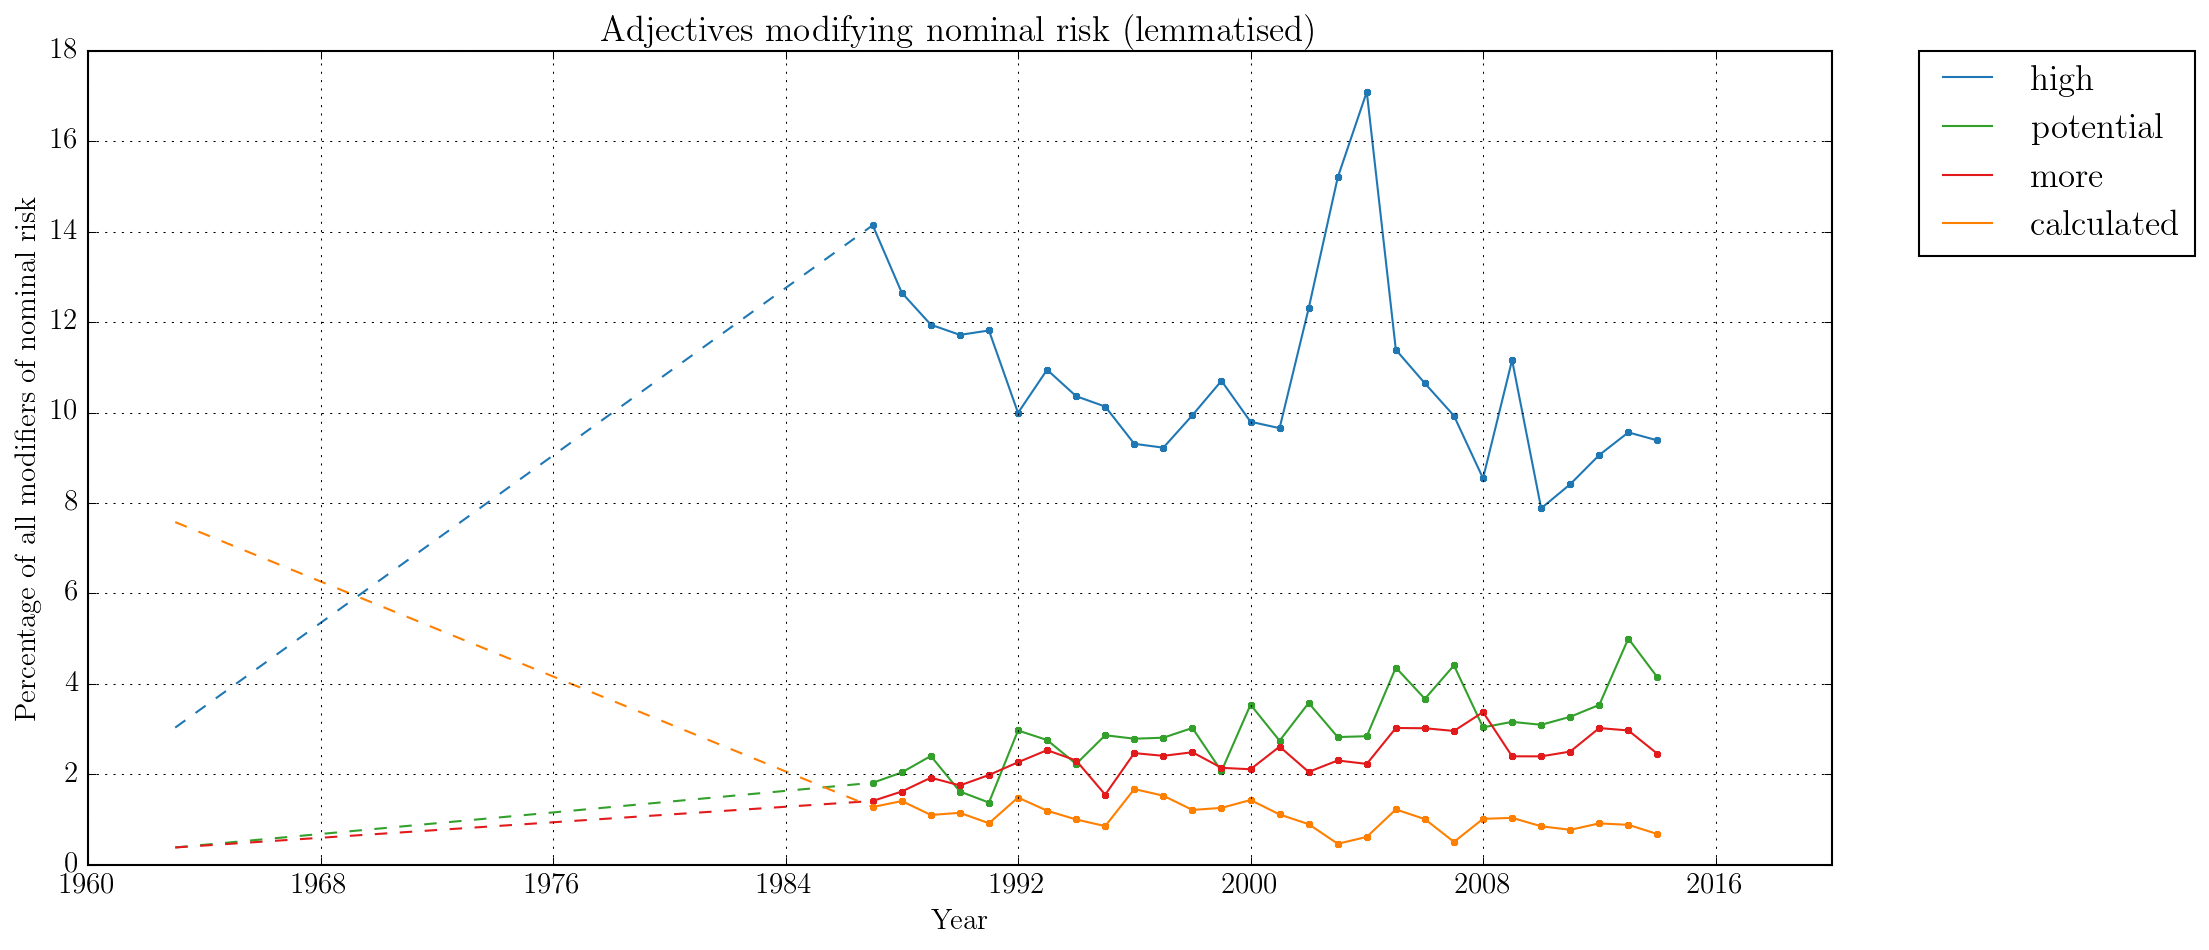
\includegraphics[width=0.75\textwidth]{../images/adjectives_modifying_nominal_risk_(lemmatised).png}
    \caption{Selected modifiers of participant risk as percentage of all risk modifiers}
    \label{fig:reladjrisk}
    \end{figure}

    %~\ \todo[inline,color=yellow!40]{\noindent Significance of this?}

    \vspace{5mm}\noindent\begin{tcolorbox}[colback=yellow!5,colframe=yellow!40!black,title=Summary: modifiers of risk as participant]
    \parbox{1\textwidth}{%
    \emph{Calculated risk} has been overtaken by \emph{potential risk} in overall frequency. \emph{High-risk} spikes in frequency in references to H5N1.}
    \end{tcolorbox}
    \vspace{5mm}


\section{What kinds of risk processes are there, and what are their relative frequencies?} \FloatBarrier

    Our second area of interest within the transitivity system is risk as a process. Within the corpus, we located five distinct risk processes. First, risk alone may be a process (\emph{I won't risk it}). Second and third are \emph{running risk} and \emph{taking risk}---\emph{process--range} configurations, where the verbal component is largely shorn of meaning, and with meaning conveyed primarily in the nominal in object position \cite{halliday_introduction_2004}. Fourth is \emph{putting somebody/something at risk}, which involves an obligatory nominal object argument and a prepositional-phrase complement. Finally, we have

    Other phrases sit on the cusp as recognisable risk processes: \emph{to carry risk}, for example, is frequent in the data, but we have not included it because we feel that the semantic burden of this process still lies in \emph{carry} (unlike \emph{pose} in \emph{to pose risk}).\endnote{Further research devoting more time to which examples constitute risk processes and which constitute experiential objects of other processes seems timely.}

    \begin{figure}[htb!]
    \centering
    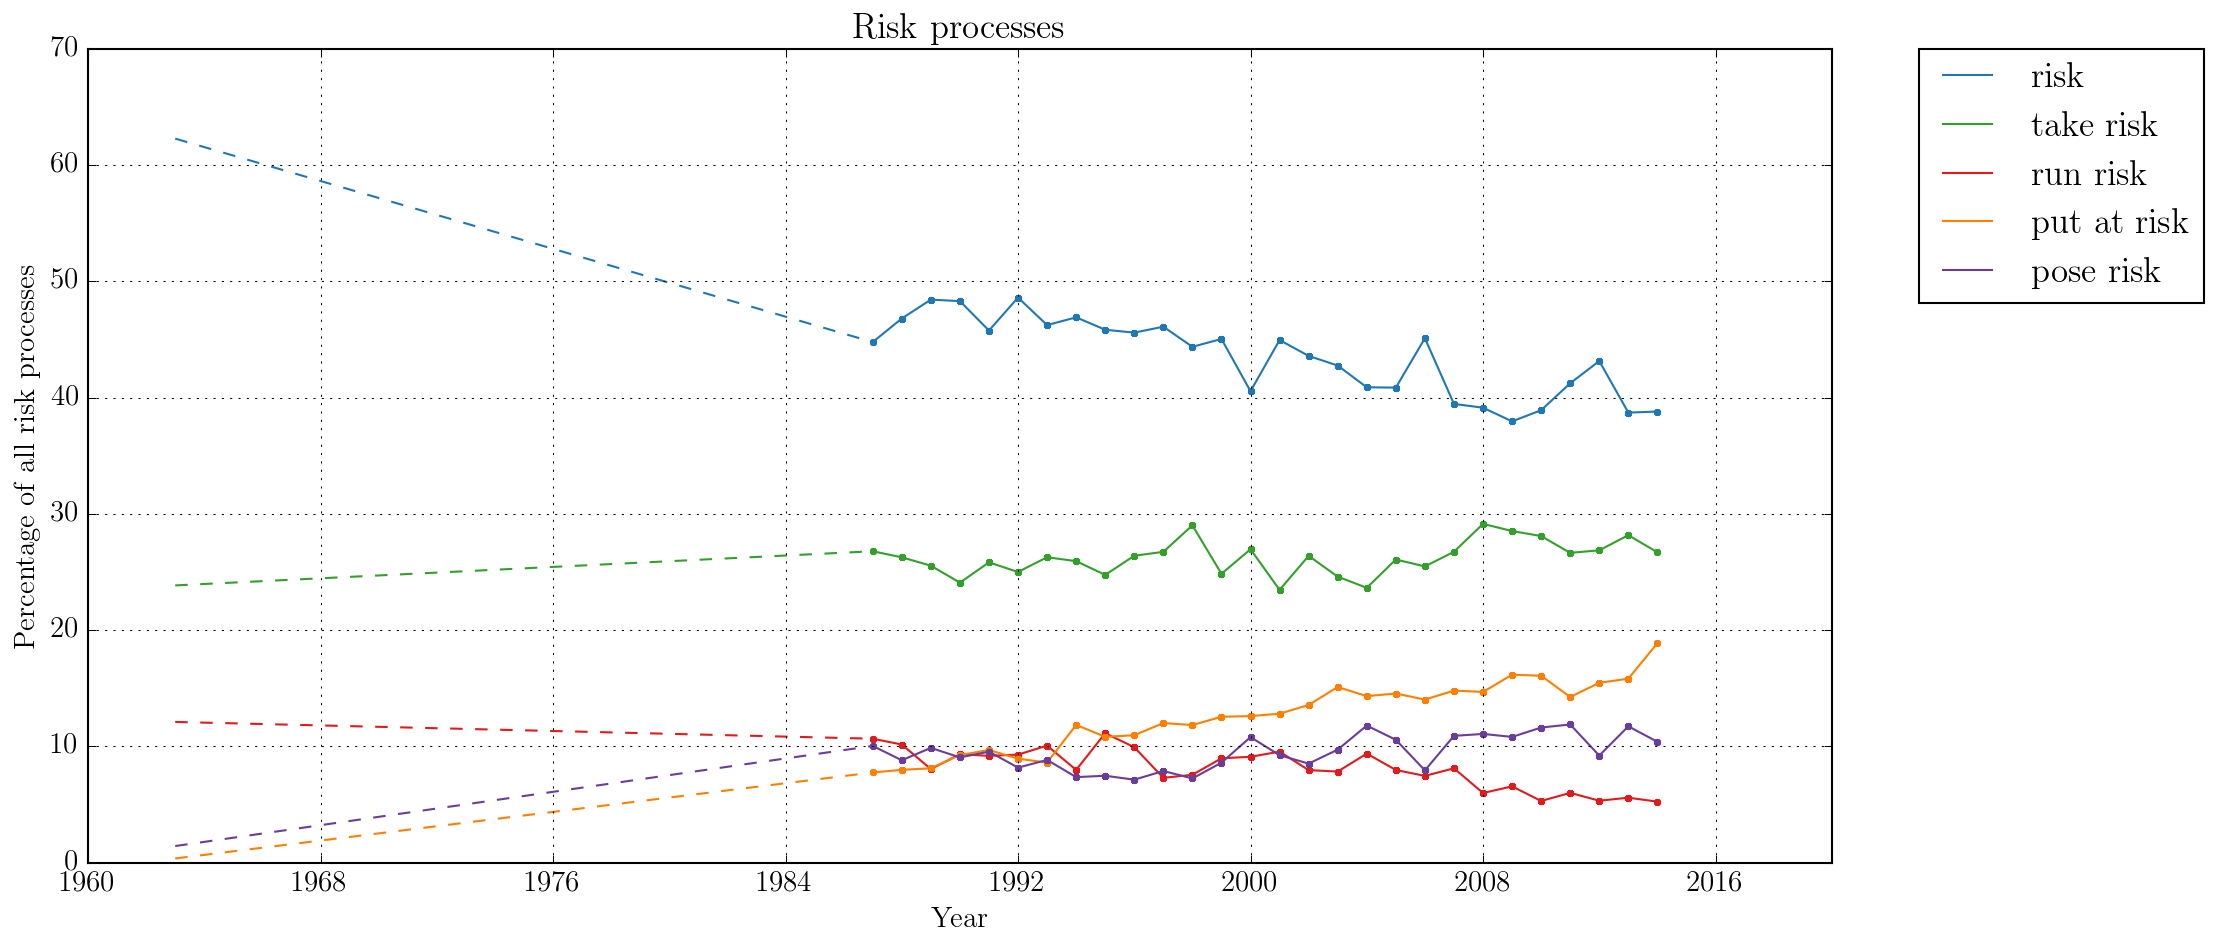
\includegraphics[width=0.75\textwidth]{../images/risk_processes.png}
    \caption{Risk processes as percentage of all parsed processes}
    \label{fig:riskprocesses}
    \end{figure}
    %
    Our first interest is the overall frequency of these five risk processes. 
    %From Figure \ref{fig:riskprocesses}, we concluded that risk processes generally are on an static\slash slightly outbound trajectory, with a notable decrease in frequency between the 1963--1987 samples.
    Figure \ref{fig:riskprocesses} charts the trajectory of the five identified risk processes. Most interesting here are that the `standard' (i.e. predicatorial) risk process is steadily decreasing, in favour of the other processes, each of which seems to provide additional connodations of the agency of the risker as well as his\slash her\slash its understanding of the level of risk. 

    The second notable finding here is that \emph{putting at risk} has overtaken \emph{running risk} in frequency. Concordancing revealed that in 2014, \emph{putting at risk} is used in cases where the potential harm is either implicit or explicit:

    \begin{enumerate}  [before=\itshape,font=\normalfont] \setlength\itemsep{0em} \small
    \item Ultimately, there is a price to pay: If you attack our soldiers, you're putting yourself at risk.
    \item But addicted health care workers need not be physicians to put patients at risk.
    \item While obviously no airline or company deliberately puts people at risk, `sometimes new risks are identified and steps have to be taken,' Mr. Koch said.
    \end{enumerate}

    \begin{enumerate}  [before=\itshape,font=\normalfont] \setlength\itemsep{0em} \small
    \item The auction houses deny that they are trimming profits with givebacks or putting themselves at financial risk.
    \item Rather, such tax status is generally put at risk when groups stray from their mission.
    \item They had handled her body, putting them at serious risk of infection.
    \end{enumerate}

    That said, we also noted that there seems to be some evidence for lessening agency in recent \emph{risk running} processes. Compare 1963 and 2014 results:

    \begin{enumerate} [before=\itshape,font=\normalfont]  \setlength\itemsep{0em} \small
    \item However, if adults decide to run a risk, this is up to them, and anyway, Switzerland adequately handles American affairs in Havana.
    \item In Washington at the weekend it was pretty welt agreed that the MIG incident was not deliberate provocation; the feeling was that, even with the Russian presence, Castro would not wilfully run the risk of American retaliation.
    \item  If he sticks to the more-or-less official Republican position against off-track betting, he runs the risk of losing thousands of New York City votes, which he needs.
    \end{enumerate}

    \begin{enumerate} [before=\itshape,font=\normalfont]   \setlength\itemsep{0em} \small
    \item Fans see this revolving door of injuries with so much regularity that they run the risk of becoming desensitized 
    \item `One runs the risk of falling for a voice.'
    \item `I would run the risk of having two boys,' she said.
    \item On the other hand, if Argentina does default, it runs the risk of more lawsuits, said Siobhan Morden, head of Latin America strategy at Jefferies.
    \item And, like an overdressed beachgoer, a classic cocktail served straight up runs a high risk of wilting in the sunshine.
    \end{enumerate}
    %
    Overall, the shift in both the semantics of risk running and the increasing preference for \emph{putting at risk} can be seen as evidence for decreasing agency in risk, as well as an increasing implicitness of the potential harm. This finding is especially significant, given that the existing descriptions of risk \cite{fillmore_toward_1992}, as well as the current FrameNet database, include accounts of \emph{running risk} as a frame, but not \emph{putting at risk}.

    \vspace{5mm}\noindent\begin{tcolorbox}[colback=yellow!5,colframe=yellow!40!black,title=Summary: types of risk processes]
    \parbox{1\textwidth}{%
    Both \emph{pose risk} and \emph{put at risk} have overtaken \emph{run risk} in frequency. Use of the prototypical risk process, \emph{to risk} is declining. Finally, there is some evidence for reduced agency the \emph{run risk} process.}
    \end{tcolorbox}
    \vspace{5mm}
    
\section{When risk is a process, what participants are involved?} \FloatBarrier
    
    Clauses containing risk processes are a rich site for analysis, as the semantic roles of participants are determined by their placement with respect to the process. In frame semantic terms, experiential subjects of risk processes can often be mapped to \emph{actors}.\endnote{A limitation of frame semantics is its ability to deal with other kinds of risk processes: in \emph{The site posed risks}, \emph{pose} is the experiential subject, but not the actor or risker.}~Experiential objects are either \emph{valued objects} or \emph{harm} (\emph{they risked their lives/death}). Table \ref{tab:riskersx} lists the most common subject and object participants of risk processes. Also of interest are clauses embedded within risk processes (e.g. \emph{she risks hurting herself\slash losing her life}). Table \ref{alienating} lists the (lemmatised) top twenty subordinated processes in the corpus.

    \begin{table}[htb!]
    \centering
    \addvbuffer[12pt 8pt]{\begin{minipage}{.35\textwidth}
    \centering
    \small
    \begin{tabularx}{1.0\textwidth}{|>{\raggedright}l|X|}
    \hline
    \textbf{Risker}           & \textbf{Risked thing\slash potential harm} \\ \hline
    person & life \\ \hline
    company & injury \\ \hline
    state & loss \\ \hline
    woman & everything \\ \hline
    man & death \\ \hline
    investor & money \\ \hline
    bush & wound \\ \hline
    player & war \\ \hline
    government & career \\ \hline
    worker & arrest \\ \hline
    republican & health \\ \hline
    clinton & damage \\ \hline
    bank & reputation \\ \hline
    democrat & fine \\ \hline
    anyone & capital \\ \hline
    obama & future \\ \hline
    child & confrontation \\ \hline
    move & job \\ \hline
    firm & backlash \\ \hline
    administration & failure \\ \hline
    \end{tabularx}
    \caption{Riskers and risked things and\slash or potential harms}
    \label{tab:riskersx}

    \end{minipage}} \hspace{1cm} % This must go next to `\end{minipage}`
    \addvbuffer[12pt 8pt]{\begin{minipage}{.35\textwidth}

    \centering
    \small
    \begin{tabularx}{0.9\textwidth}{|l|X|}
    \hline
    \textbf{Embedded process}      & \textbf{Total ~~~~~~~~~~~~~~~~~~~~~~~~~~~~~~~~~~~~~~~~~~} \\ \hline
    lose      & 1260  \\ \hline
    be        & 1095  \\ \hline
    alienate  & 379   \\ \hline
    have      & 347   \\ \hline
    become    & 285   \\ \hline
    get       & 184   \\ \hline
    make      & 166   \\ \hline
    turn      & 119   \\ \hline
    go        & 113   \\ \hline
    offend    & 110   \\ \hline
    take      & 86    \\ \hline
    look      & 85    \\ \hline
    undermine & 82    \\ \hline
    anger     & 79    \\ \hline
    fall      & 78    \\ \hline
    create    & 76    \\ \hline
    put       & 74    \\ \hline
    miss      & 73    \\ \hline
    give      & 73    \\ \hline
    damage    & 62    \\ \hline
    \end{tabularx}
    \caption{Most common embedded processes in risk processes}
    \label{alienating}
    
    \end{minipage}}
    \end{table}

    Riskers are most typically powerful institutions or individuals. Risked things and potential harms are generally serious and grave. A mismatch occurs here: \emph{Bush} and \emph{Obama} do not likely risk \emph{wounds}, \emph{arrest} or \emph{death}. In terms of subordinated processes, notable is the appearance of processes that are fairly uncommon: \emph{alienating}, \emph{offending}, \emph{undermining} and \emph{angering} and are three key examples, ranking amongst expected processes like \emph{being}, \emph{having}, \emph{getting}, \emph{making} and \emph{going}. Without considering longitudinal change, we can see from this that the embedded processes are often related to more powerful social actors: states, political parties and politicians risk alienating electorates; diplomats risk offending one another. Even embedded processes lacking explicit connotations of power are typically deployed in the contexts of government, industry or society. Below are concordance results for \emph{risk alienating} in 2013, which appears 14 times.

    \begin{figure}
    \footnotesize
    \begin{tabular}{rcl}
    stoked further concerns that unemployment risked &  becoming &  endemic and could eventually cause social upheaval  \\ 
    franchise, the stage scene could have risked &  becoming &  an embarrassment for the brand, but Mr. Timbers'   \\ 
    with locally, or else the Vatican offices risk &  becoming &  institutions of censorship   \\ 
    on which the experience depends -- or risk &  becoming &  irrelevant to future generations, Mr. Staggs said   \\ 
    restart growth, warning that the euro area risked &  becoming &  mired in the same kind of economic stagnation that   \\ 
    If left unaddressed, such practices risk &  becoming &  more and more entrenched, Ann Harrison of   \\ 
    without serious savings in this area, we risk &  becoming &  an unbalanced force, one that is well compensated   \\ 
    Switzerland risks &  becoming &  one of the most restrictive places for management   \\ 
    What was the exception before now risks &  becoming &  the standard practice   \\ 
    the pope's new remarks that the church risked &  becoming &  a `small chapel' overly fixated on sexual   \\ 
    hailed the step as significant, it risks &  becoming &  the latest of many tentative moves toward talks   \\ 
    Rather than race the clock to Bed-Stuy and risk &  becoming &  an early bike-share casualty, I stopped at a   \\ 
    increasingly turning to what, strangely, risked &  becoming &  the most marginalized group of all: the bosses   \\ 
    and currency crisis in the European Union risks &  becoming &  a crisis of liberal democracy itself \\ 
    \end{tabular}
    \caption{\emph{To risk becoming} in 2013 subcorpus}
    \end{figure}

    \begin{figure}[htb!]
    \centering
    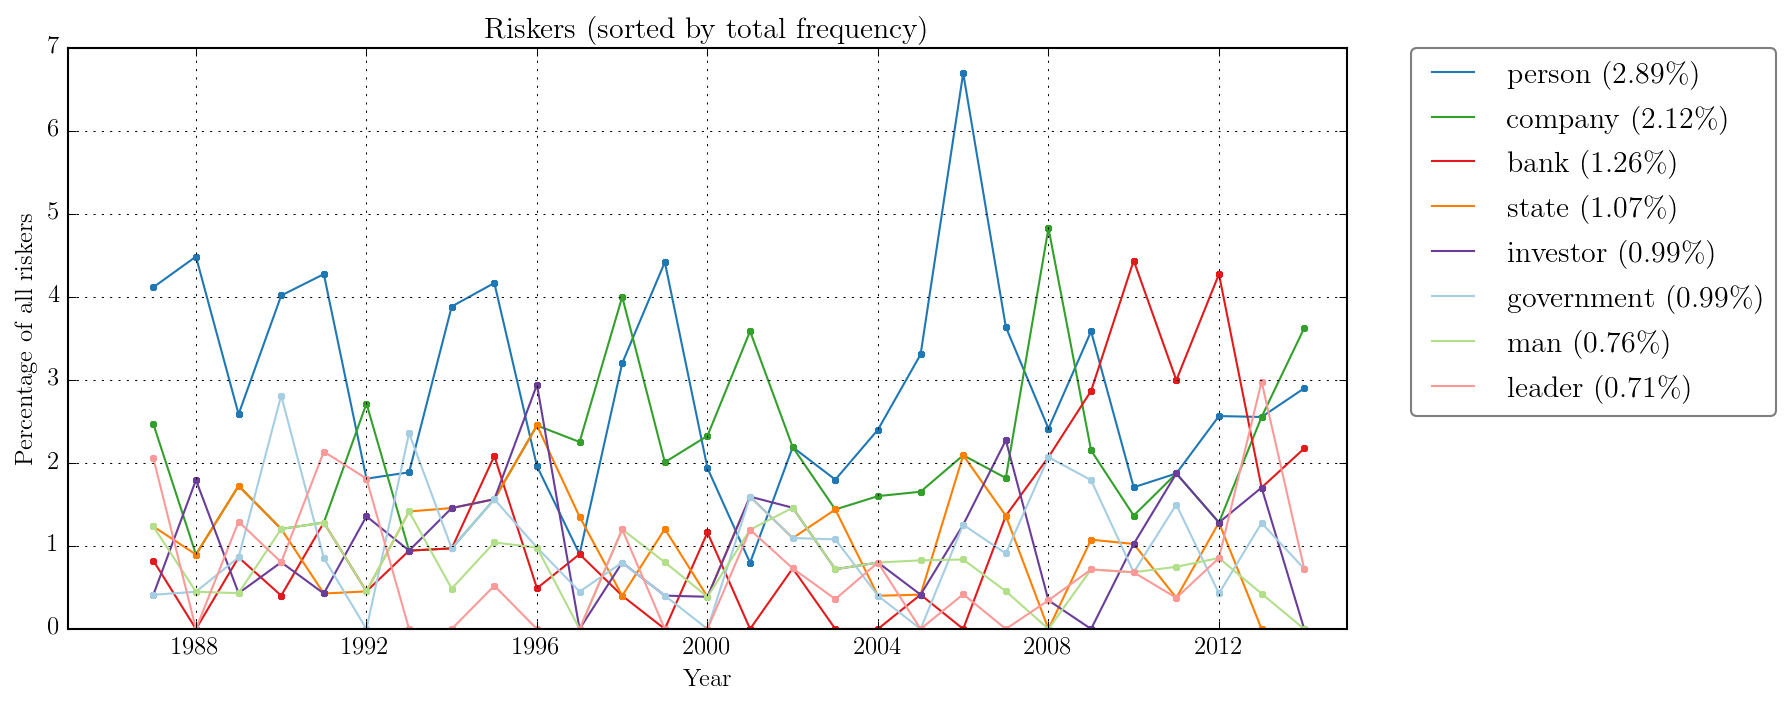
\includegraphics[width=0.75\textwidth]{../images/riskers-sorted-by-total-frequency.png}
    \caption{Riskers, sorted by total frequency}
    \label{fig:riskers}
    \end{figure}

    There is some evidence everyday people are less commonly riskers in later editions: if we sort the `riskers' (Figure \ref{fig:riskers}) by those that are decreasing at the fastest rate over the course of our dataset, \emph{man\slash men}, \emph{woman\slash women} and \emph{person\slash people} are all in the top seven. Conversely, when sorting by those on the most upward trajectory, the lemmas \emph{bank}, \emph{company}, \emph{firm} and \emph{agency} are in the top seven (Figure \ref{fig:increase_decrease_riskers}). Further findings in this vein are presented in more depth in Zinn \& McDonald, 2015.

    \noindent
    \begin{figure}[htb!]
    \centering
    \begin{minipage}{.48\textwidth}
    \centering
    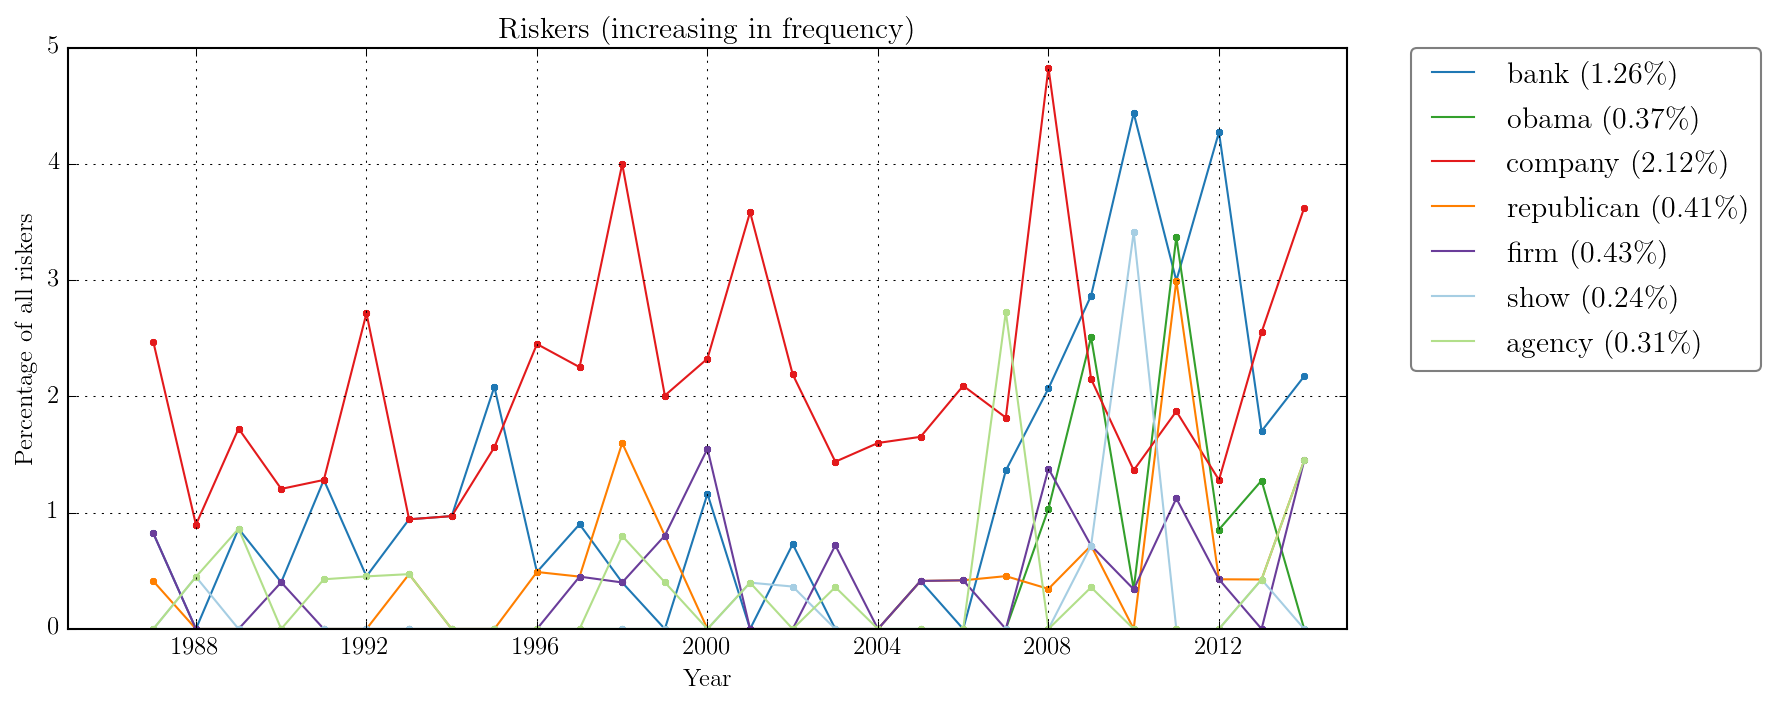
\includegraphics[width=0.98\textwidth]{../images/riskers-increasing-in-frequency.png}
    \end{minipage}%
    \begin{minipage}{.48\textwidth}
    \centering
    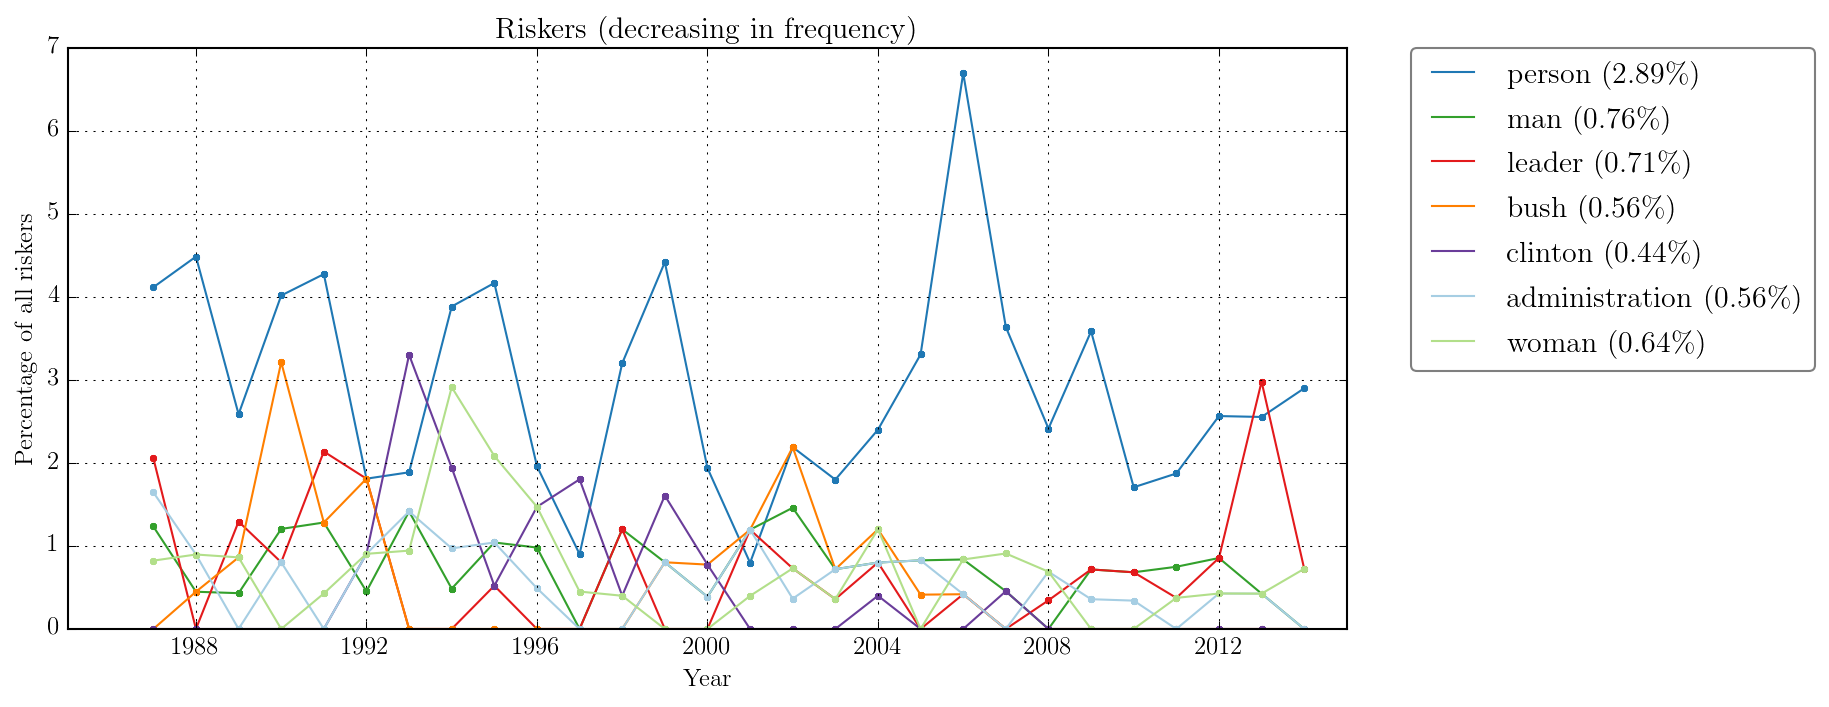
\includegraphics[width=0.98\textwidth]{../images/riskers-decreasing-in-frequency.png}
    \end{minipage}
    \caption{Riskers, sorted by most increasing (left) and most decreasing (right)}
    \label{fig:increase_decrease_riskers}
    \end{figure}

    %Though these objects may be grammatically ambiguous, the function of the object can be disambiguated by inserting \emph{losing}.

    %\begin{enumerate}	\setlength\itemsep{0em}
    %\item He risked his life
    %\item He risked losing his life
    %\item He risked death
    %\item * He risked losing death
    %\end{enumerate}

    %Note here an emerging methodological issue: the various  \emph{potential harms} can also be located by querying nominal risks (e.g. \emph{the risk of death}). Some methodological adaptability is thus required.

    \vspace{5mm}\noindent\begin{tcolorbox}[colback=yellow!5,colframe=yellow!40!black,title=Summary: participants in risk processes]
    \parbox{1\textwidth}{%
    When risk is a process, risked things\slash potential harms often pertain to individual health (\emph{to risk life, death, health, etc.}). This contrasts with processes as potential harm, which generally relate to people in positions of power (\emph{to risk alienating voters}, for example).}
    \end{tcolorbox}
    \vspace{5mm}

\section{When risk is a modifier, what are the most common forms?} \label{sect:mod_one} \FloatBarrier

    \begin{table}
    \small
    \centering
    \begin{tabular}{|l|l|}
    \hline
    \textbf{Modifier type}       & \textbf{Example}          \\ \hline
    Adjectival pre-head & \emph{a risky move}     \\ \hline
    Post-head           & \emph{A person at risk} \\ \hline
    pre-head nominal    & \emph{risk management}  \\ \hline
    Adverbial           & \emph{to riskily act}   \\ \hline
    Circumstance head   & \emph{to be at risk }   \\ \hline
    \end{tabular}
    \caption{Types of risk-as-modifier}
    \label{tab:modriskwords}
    \end{table}

    There are many different kinds of risk as modifier (see Table \ref{tab:modriskwords} for a non-exhaustive list of examples). Our first interest was in gauging the prevalence of the different forms. From this query, we noted that pre-head nominal modifiers are increasing in frequency. A good example is \emph{risk factor} (see Figure \ref{fig:riskfactor}).

    \noindent
    \begin{figure}[htb!]
    \centering
    \begin{minipage}{.567\textwidth}
    \centering
    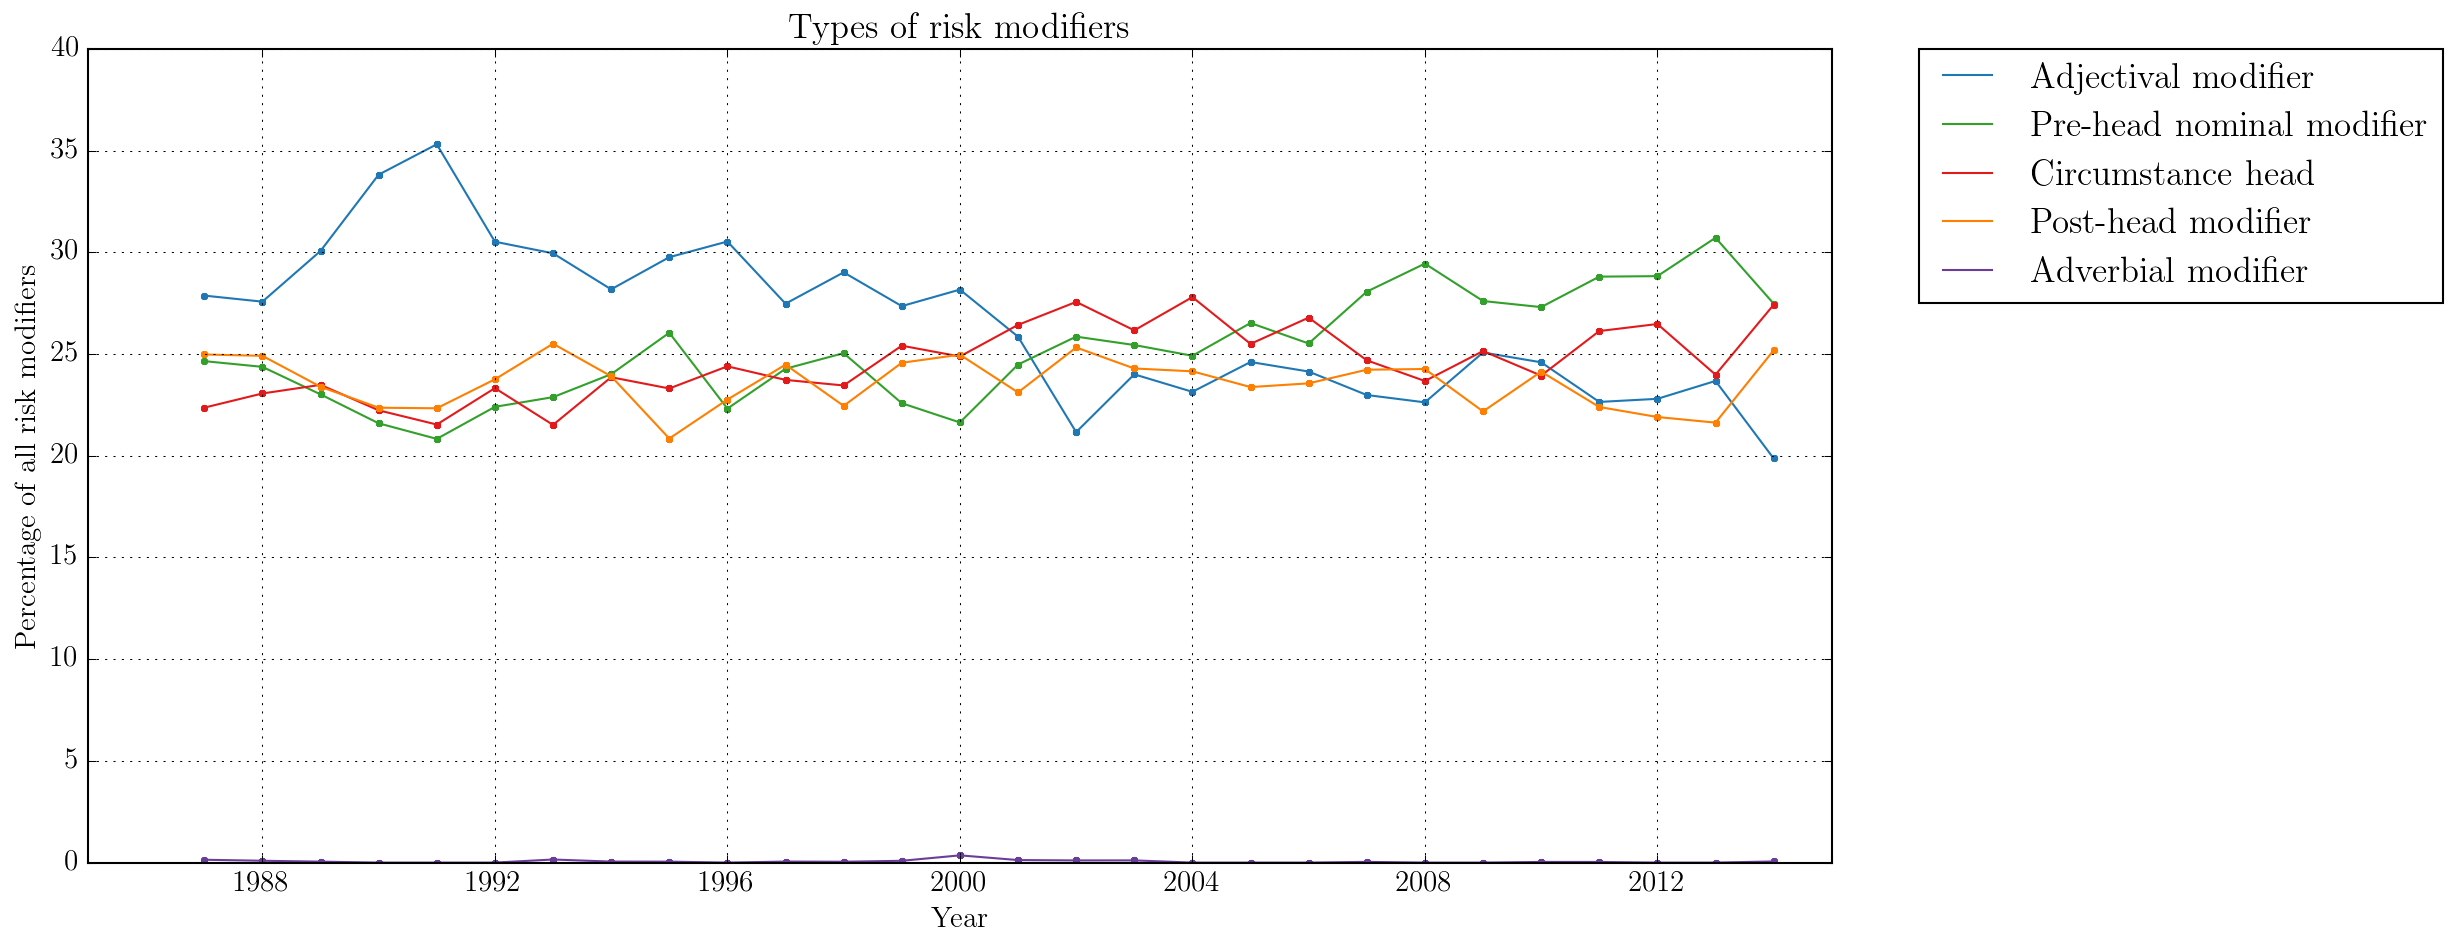
\includegraphics[width=0.98\textwidth]{../images/types-of-risk-modifiers.png}
    \captionof{figure}{Types of risk modifier}
    \label{fig:riskmod_types}
    \end{minipage}%
    \begin{minipage}{.433\textwidth}
    \centering
    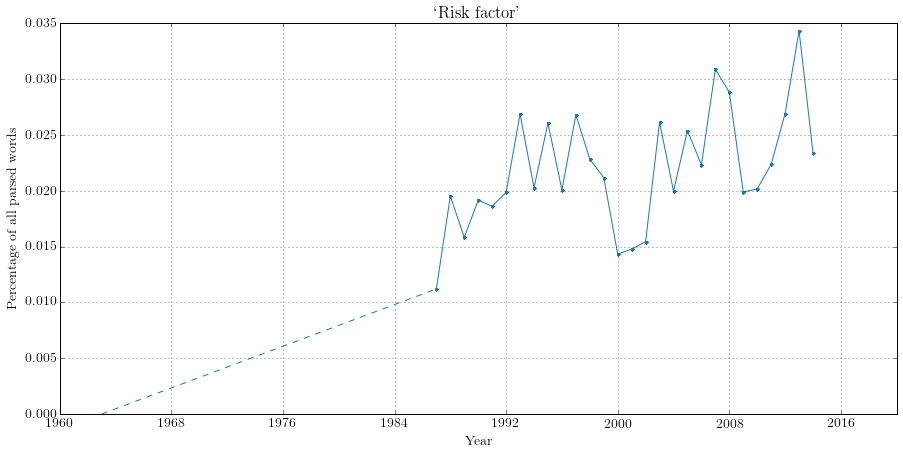
\includegraphics[width=0.98\textwidth]{../images/risk-factor.png}
    \captionof{figure}{Relative frequency of \emph{risk factor}}
    \label{fig:riskfactor}
    \end{minipage}
    \end{figure}


    Modifier risks are unique for their variety and diversity: through compounding, comprehensible new risk words and phrases can easily be created. The entire corpus contained 327 unique adjectival risk words, including \emph{non-risk}, \emph{de-risk}, \emph{once-risky}, \emph{take-no-risks}, \emph{risk-swapping}, \emph{risk-abhorrent}, \emph{price-for-risk}, \emph{post-risky}, \emph{pooled-risk}, \emph{personal-risk}, \emph{optimum-risk}, \emph{one-risk-factor}, \emph{one-pitch-can-end-his-career-risk} and \emph{low-risk-to-society}. That said, most of these occur no more than a handful of times. By far the most common were \emph{risky\slash riskier\slash riskiest} (15588 occurrences), \emph{high-risk} (5533), \emph{low-risk} (1086), \emph{at-risk} (902), \emph{risk-free} (883) and \emph{risk-taking} (789). Of these, four exhibited trajectory shifts (see Figure \ref{fig:adjtraj}). The basic adjectival forms (\emph{risky}, \emph{riskier}, \emph{riskiest}) are dominant in the 1963 sample, then decrease, and re-emerge in 2000. \emph{High-risk} though very rare (two instances) in 1963, has become more common, and stabilised in trajectory. \emph{Low-risk} and \emph{at-risk} are on a consistent inbound trajectory.

    \noindent
    \begin{figure}[htb!]
    \centering
    \begin{minipage}{.48\textwidth}
    \centering
    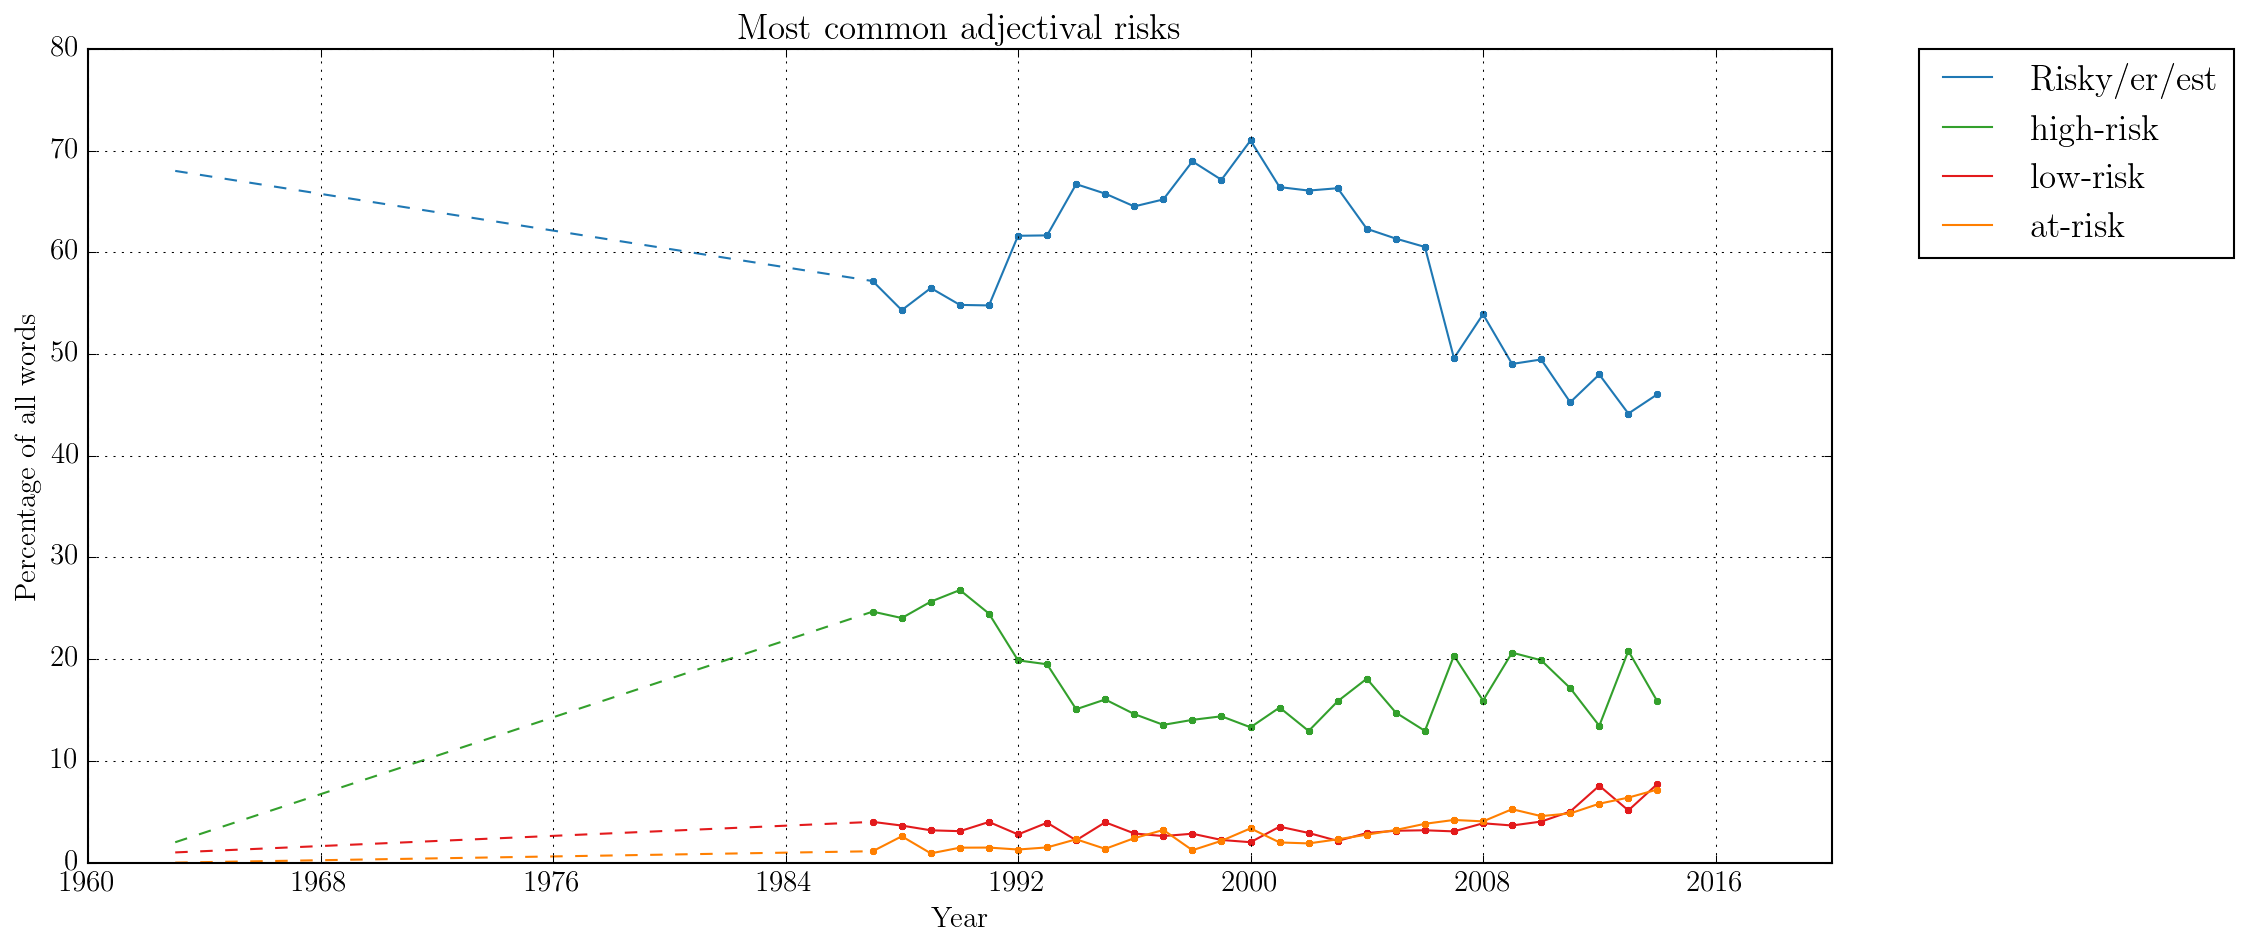
\includegraphics[width=0.98\textwidth]{../images/most_common_adjectival_risks.png}
    \end{minipage}%
    \begin{minipage}{.48\textwidth}
    \centering
    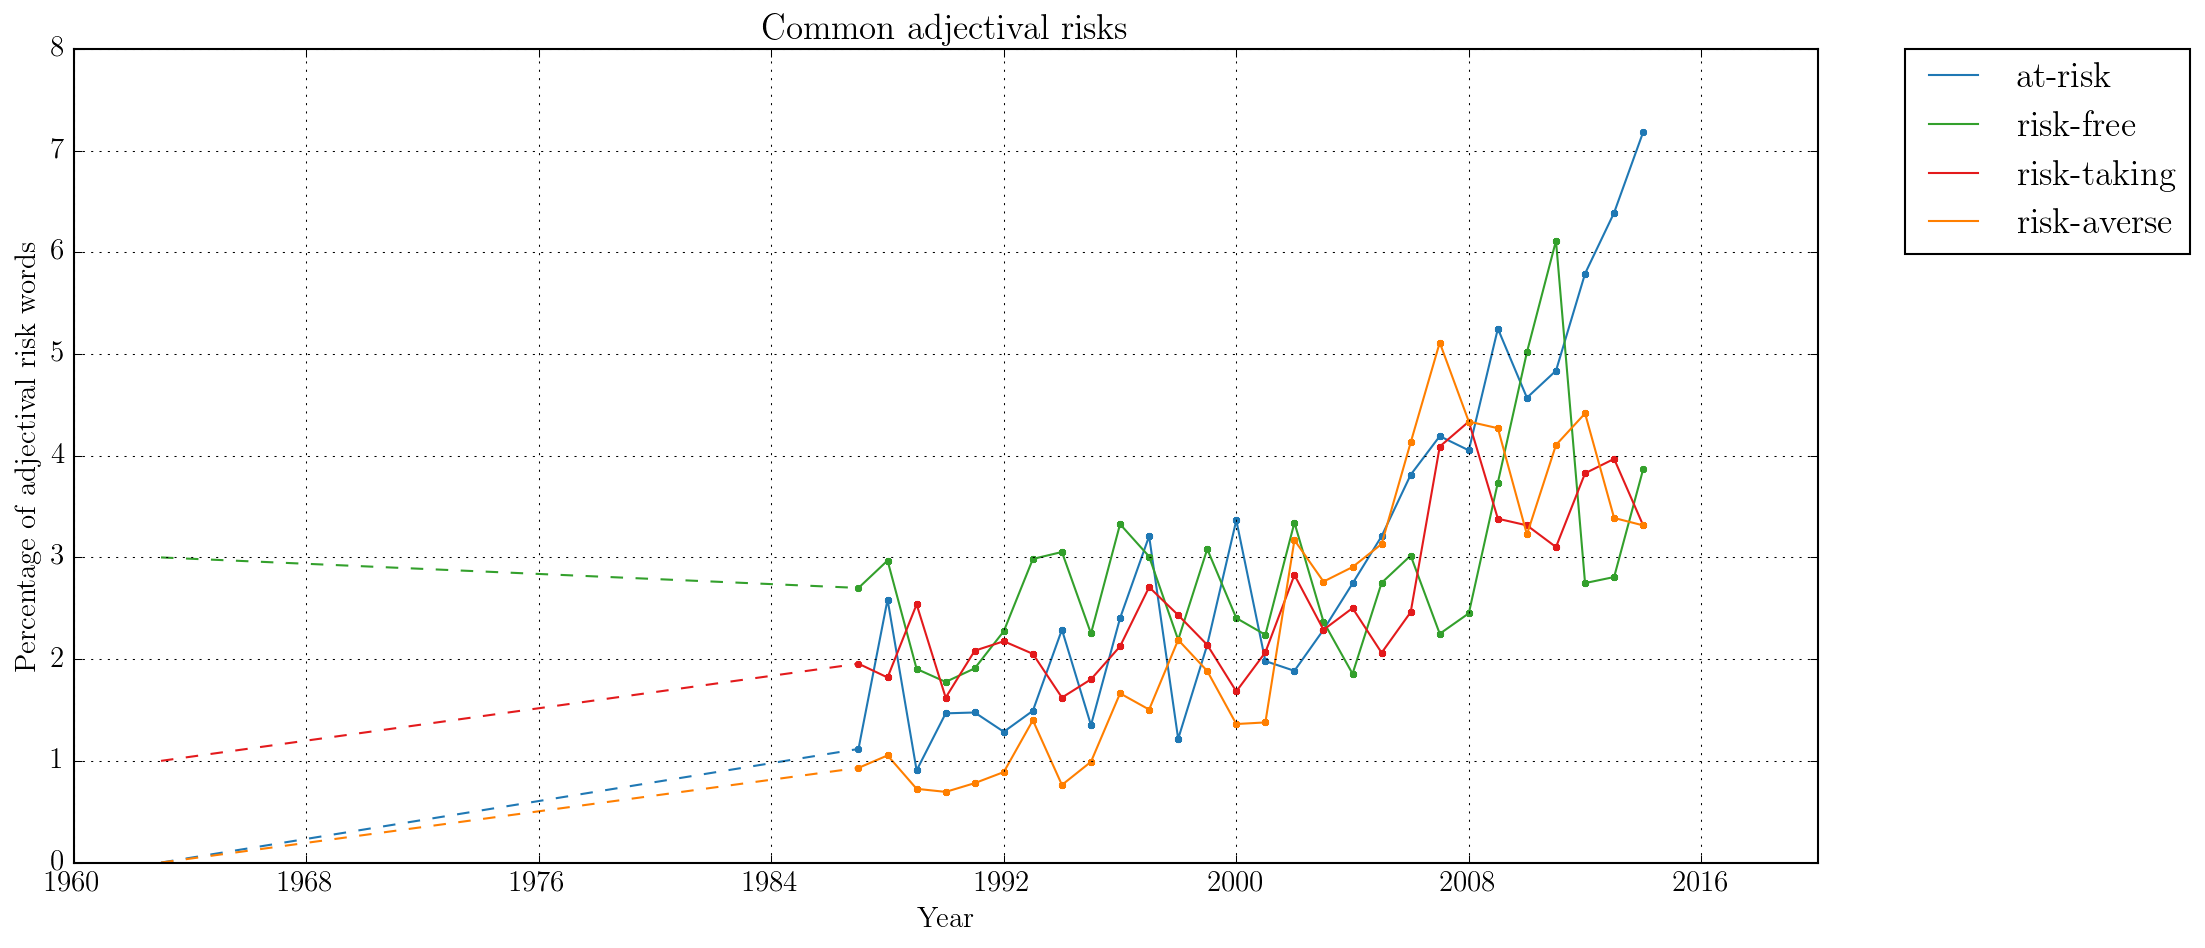
\includegraphics[width=0.98\textwidth]{../images/common_adjectival_risks.png}
    \end{minipage}
    \caption{Common adjectival risk words as percentage of all adjectival risks}
    \label{fig:adjtraj}
    \end{figure}

    The prevalence of \emph{high-risk} in the 1980s is largely due to the AIDS epidemic: concordancing reveals that certain populations (gays, African Americans, Haitians) are at high-risk of being inflected by HIV. \emph{At-risk} is rare in earlier editions, but increases in prevalence steadily. This shift in risk is modifier is an important one. \emph{Low-}, \emph{moderate-} and \emph{high-risk} comprises a gradient, or scale, while \emph{at-risk} is a binary. As with the shift toward \emph{potential risk}, this indicates both an increasing pervasiveness and a decreasing calcuability of risk. %remember that low-risk is actually increasing.
    
    %Of the graduated risks, low-risk is the only one on an inbound trajectory. What's the significance of this?



    %For people at moderate risk who also have two of the other risk factors , the treatment should be the same as for those in the high-risk group .
    %But ecologists , doctors and other specialists here warn that the entire population , not just high-risk groups , is vulnerable .
    %In the weeks since the law took effect , couples seeking marriage licenses have besieged hospitals , clinics and other doctors , anxious to get the test and the required counseling in time for wedding dates and quickly outnumbering those in high-risk groups most in need of attention .
    %Health experts say scarce funds for AIDS prevention would be better spent on high-risk groups .
    %Very few Americans know that Haitians have long since been removed from the list of high-risk groups because it was discovered that the H

    \vspace{5mm}\noindent\begin{tcolorbox}[colback=yellow!5,colframe=yellow!40!black,title=Summary: frequencies of modifier risk]
    \parbox{1\textwidth}{%
    Common risk modifiers (\emph{risky}, \emph{riskier}, \emph{riskiest}) are gradually being displaced by a number of less common constructions (e.g. \emph{low-risk}, \emph{at-risk}, \emph{risk-averse}, \emph{risk-free}).}
    \end{tcolorbox}
    \vspace{5mm}

\section{When risk is a modifier, what is being modified?} \label{sect:mod_two} \FloatBarrier 

    Risk as a modifier can be placed either before or after the noun it modifies (\emph{an at-risk person\slash a person at risk}). These two constructions are collapsed in Tables \ref{tab:riskmodified} and \ref{tab:atrisk}, which respectively list the participants most frequently modified by any risk modifier, and the participants most frequently modified by \emph{at-risk\slash at risk}. Note that while risk-modified participants generally are financial and economic in nature (\emph{investment, business, loan, asset}), the at-risk subset is mainly comprised of vulnerable populations of people (\emph{women}, \emph{children}, \emph{students}).

    \begin{table}[htb!]
    \centering
    \addvbuffer[12pt 8pt]{\begin{minipage}{.37\textwidth}
    \centering
    \small
    \begin{tabularx}{1.0\textwidth}{|X|l|}
    \hline
    \textbf{Risk-modified \mbox{participant}}        & \textbf{Total} \\ \hline
    investment  & 696   \\ \hline
    business    & 515   \\ \hline
    behavior    & 508   \\ \hline
    group       & 466   \\ \hline
    loan        & 421   \\ \hline
    asset       & 388   \\ \hline
    strategy    & 377   \\ \hline
    bond        & 346   \\ \hline
    area        & 307   \\ \hline
    venture     & 301   \\ \hline
    security    & 287   \\ \hline
    patient     & 265   \\ \hline
    pool        & 239   \\ \hline
    bet         & 214   \\ \hline
    move        & 204   \\ \hline
    activity    & 201   \\ \hline
    proposition & 199   \\ \hline
    child       & 170   \\ \hline
    woman       & 161   \\ \hline
    student     & 158   \\ \hline
    \end{tabularx}
    \caption{Most common risk-modified participants in the corpus}
    \label{tab:riskmodified}
    \end{minipage}} \hspace{1cm}
    \addvbuffer[12pt 8pt]{\begin{minipage}{.37\textwidth}
    \small
    \begin{tabularx}{1.0\textwidth}{|X|l|}
    \hline
    \textbf{At-risk \mbox{participant}}       & \textbf{Total} \\ \hline
    person     & 439   \\ \hline
    child      & 368   \\ \hline
    woman      & 209   \\ \hline
    student    & 179   \\ \hline
    nation     & 135   \\ \hline
    patient    & 110   \\ \hline
    youngster  & 93    \\ \hline
    group      & 91    \\ \hline
    population & 64    \\ \hline
    family     & 58    \\ \hline
    kid        & 50    \\ \hline
    youth      & 48    \\ \hline
    money      & 48    \\ \hline
    worker     & 45    \\ \hline
    life       & 41    \\ \hline
    job        & 41    \\ \hline
    man        & 40    \\ \hline
    area       & 35    \\ \hline
    teenager   & 32    \\ \hline
    other & 32 \\ \hline
    \end{tabularx}
    \caption{Most common at-risk participants in the corpus}
    \label{tab:atrisk}
    \end{minipage}}% This must go next to `\end{minipage}`
    \end{table}

    In need of further research is whether or not the list of entities that can sensibly be modified by \emph{at-risk} is beginning to grow: since the U.S. subprime mortgage crisis (beginning in 2007), references to \emph{at-risk homeowners} appear to be on the rise. Results from 2011, for example, show that \emph{nations} and even \emph{economic sectors} are being modified with \emph{at-risk}:

    \begin{enumerate}  [before=\itshape,font=\normalfont] \setlength\itemsep{0em} \small
    \item Mr. Obama asked for \$400 million for the World Bank's clean technology fund, \$95 million for the bank's program to prevent deforestation and \$90 million for its program to help at-risk nations cope with the effects of a warming planet by, for instance, developing drought-resistant crops.
    \item The most at-risk sectors included auto components and automobile companies, which generate nearly 30 percent of their sales in Europe, as well as food and tobacco firms.
    \end{enumerate}

    Note that it is difficult to reconcile the semantic meaning of \emph{at-risk} constructions with the semantic frame of risk provided by \citeA{fillmore_toward_1992}. Though elements of both the \textsc{victim} and \textsc{valued object} appear to be at work, neither provides an adequate label for \emph{at-risk people, children, homeowners or nations}. Rather than being an oversight during the articulation of the risk frame (recall Figure~\ref{fig:fil_atk}), in light of the increased use of these kinds of constructions since the mid 1990s, we hypothesise that \emph{at-risk} constructions (as well as \emph{to put at risk}) are demonstrative of a broader shift in risk discourse toward general clusters of negative outcomes, rather than specific and measurable potential harms. Connection between this shift and sociological theory is made in the following chapter.

    \vspace{5mm}\noindent\begin{tcolorbox}[colback=yellow!5,colframe=yellow!40!black,title=Summary: participants modified by risk]
    \parbox{1\textwidth}{%
    While risk as a modifier is often used in the context of finance\slash commerce, \emph{at-risk} typically attaches to vulnerable human demographics.}
    \end{tcolorbox}
    \vspace{5mm}

\section{How arguable is risk?} \label{sect:arguability} \FloatBarrier

    As noted earlier, our central concern with the Mood system is the degree of arguability associated with the concept of risk. Risk in Subject, Finite and Predicator positions is the most arguable. Risk words within Complements and Adjuncts are less arguable.

    %A dependency grammar attempts to locate a lexical root for each clause, and attach dependents to it recursively until no lexical items are unattached. Each word is ordered by its dependency to the root of a clause. The nature of the dependency relationship can also be provided. Such grammars are particularly useful for free word order language, but have been applied to English successfully as well.

    Based on the kinds of parsing provided by Stanford CoreNLP, it was possible to measure arguability in two ways. First, we can map dependency relationships to the systemic-functional notion of arguability. A dependency grammar locates the predicator of a clause and assigns it a position of zero. A `1' is then assigned to its most immediate dependent (other components in the verbal group, if present, or the head of the Subject, if not). This process continues until no lexical items are unattached, or `ungoverned'. In effect, the higher the number attached to a word, the further it is semantically from being an important component in the meaning, and thus, in systemic functional terms, the less arguable the word.

    \begin{figure}[htb!]
    \centering
    \addvbuffer[12pt 8pt]{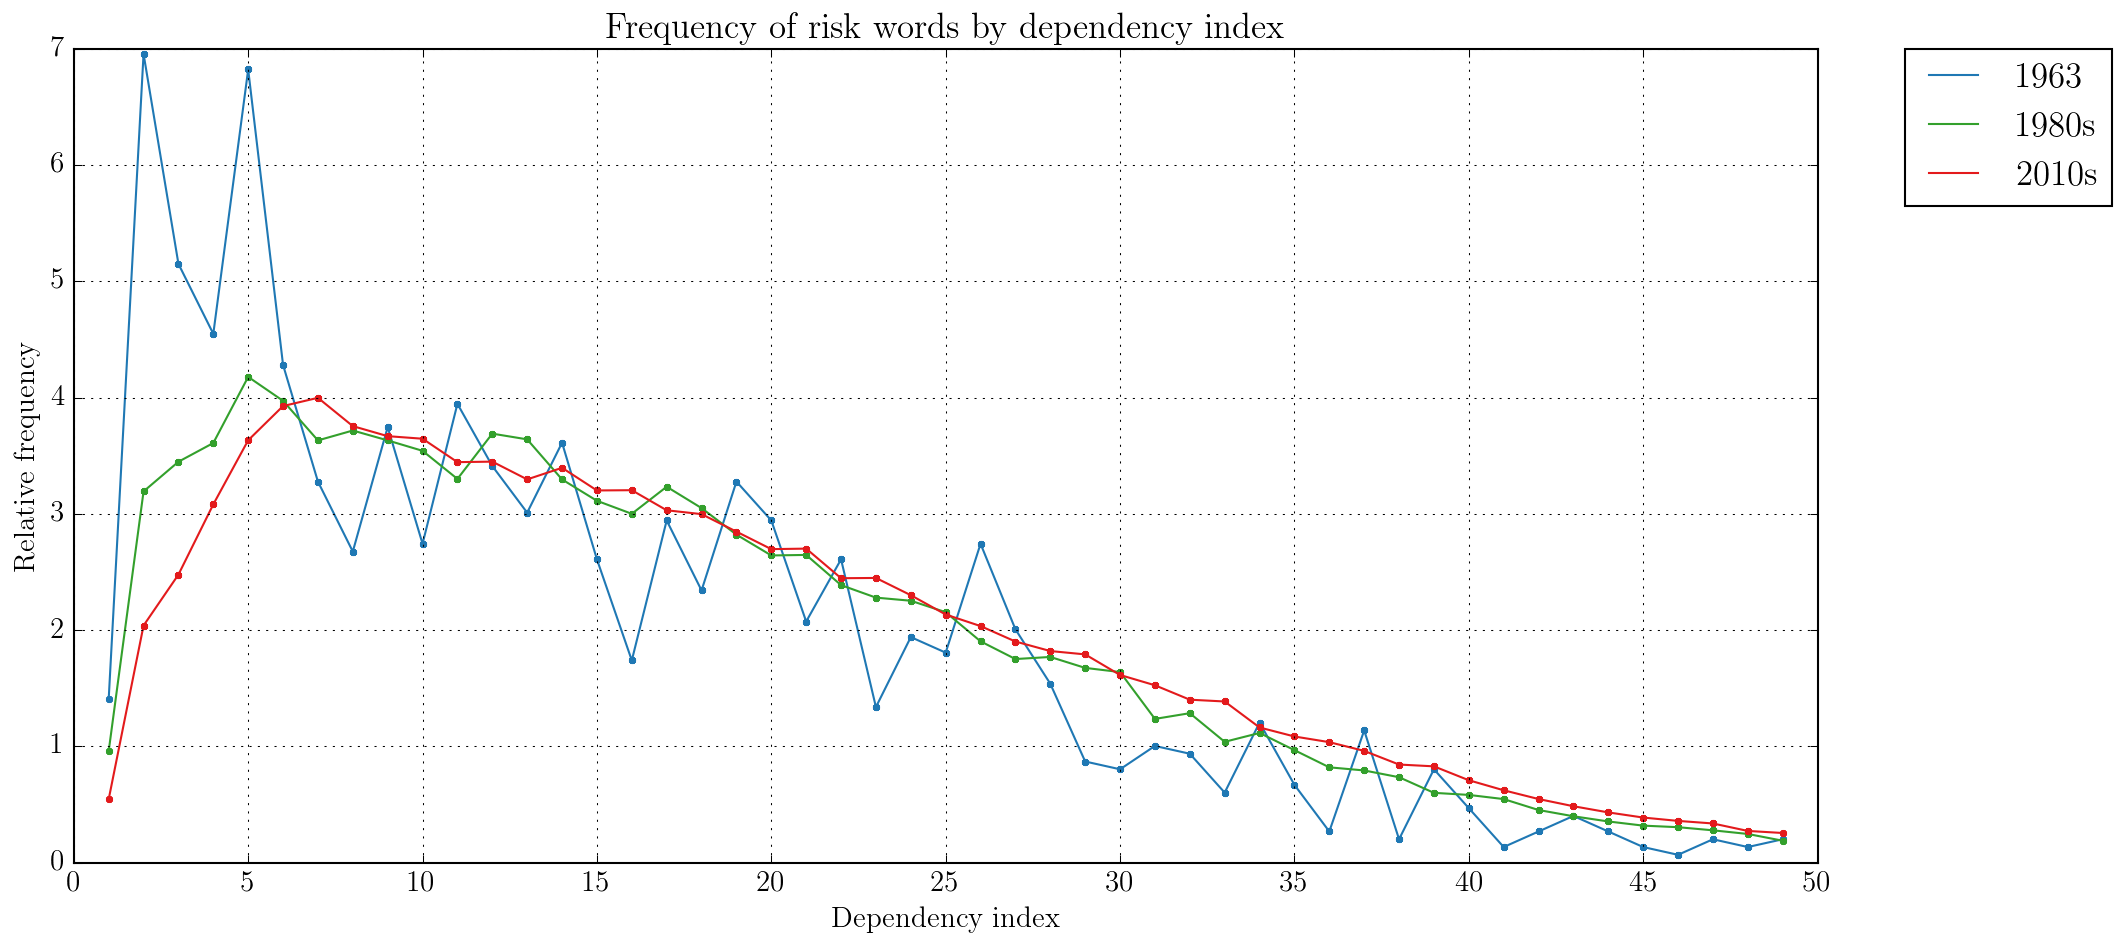
\includegraphics[width=0.75\textwidth]{../images/frequency-of-risk-words-by-dependency-index.png}}
    \caption{Risk words by dependency position in clause}
    \label{fig:depnum}
    \end{figure}
    %
    Highlighting three sampling periods as in Figure \ref{fig:depnum} shows that in early samples, risk occupies core roles within the dependency hierarchy, and thus sits closer to the core part of the meaning being exchanged within the clause. In later samples, risk more commonly occurs later in the dependency structure, in less focial positions. As explained earlier, though this experimental method is not a perfectly reliable indicators of arguability, it does indicate an increasing preference to position risk as non-core, ancillary information, rather than as the main thing which is under discussion.

    %\endnote{Dependency place 2 and 3 removed from visualisation, as these roles are typically for finites and modal auxiliaries---positions that a risk word cannot grammatically fill.}

    The second thing we can use dependency output for is identifying the functional roles of risk words. This is more accurate than using the dependency ranking, but creates a long list of functional roles. Of key interest, however, are risk words at the head of each major component of the Mood system---Subject, Finite\slash Predicator, Complement and Adjunct (CoreNLP parses unfortunately do not distinguish between Finite and Predicator in a reliable way, so the categories are collapsed here). From Figure \ref{fig:interpersonalarg}, we can see that risk is shifting from Subject and Finite\slash Predicator to Complement and Adjunct roles. This is an important result: risk words in more arguable roles are steadily decreasing, while risk in less arguable roles are becoming more common. Like earlier findings, this suggests an increasing implicitness of risk in NYT discourse, with less talk actually \emph{about} risk, but more talk where the relationship between risk and the subjects of the talk is assumed to be more or less common knowledge.

    \noindent
    \begin{figure}[htb!]
    \centering
    \begin{minipage}{.48\textwidth}
    \centering
    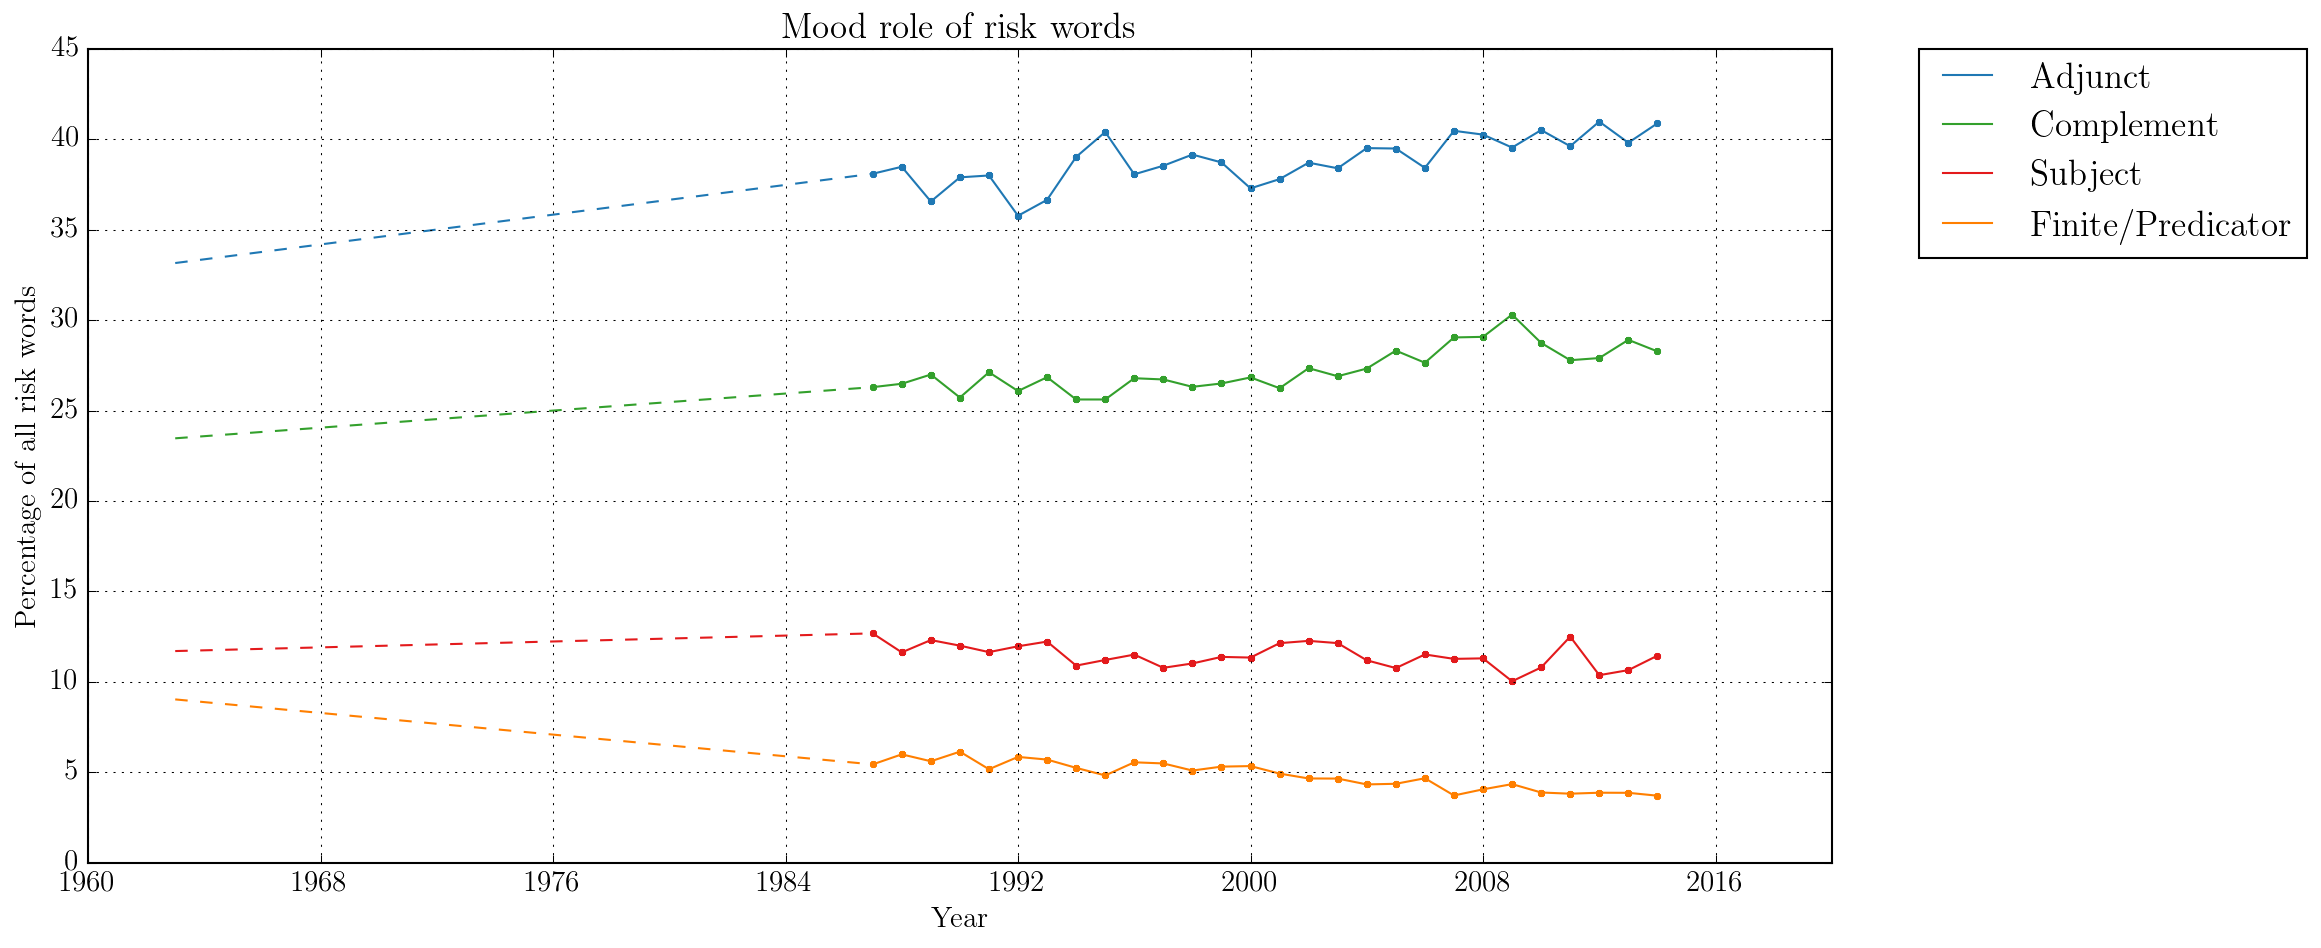
\includegraphics[width=0.98\textwidth]{../images/mood_role_of_risk_words.png}
    \end{minipage}%
    \begin{minipage}{.48\textwidth}
    \centering
    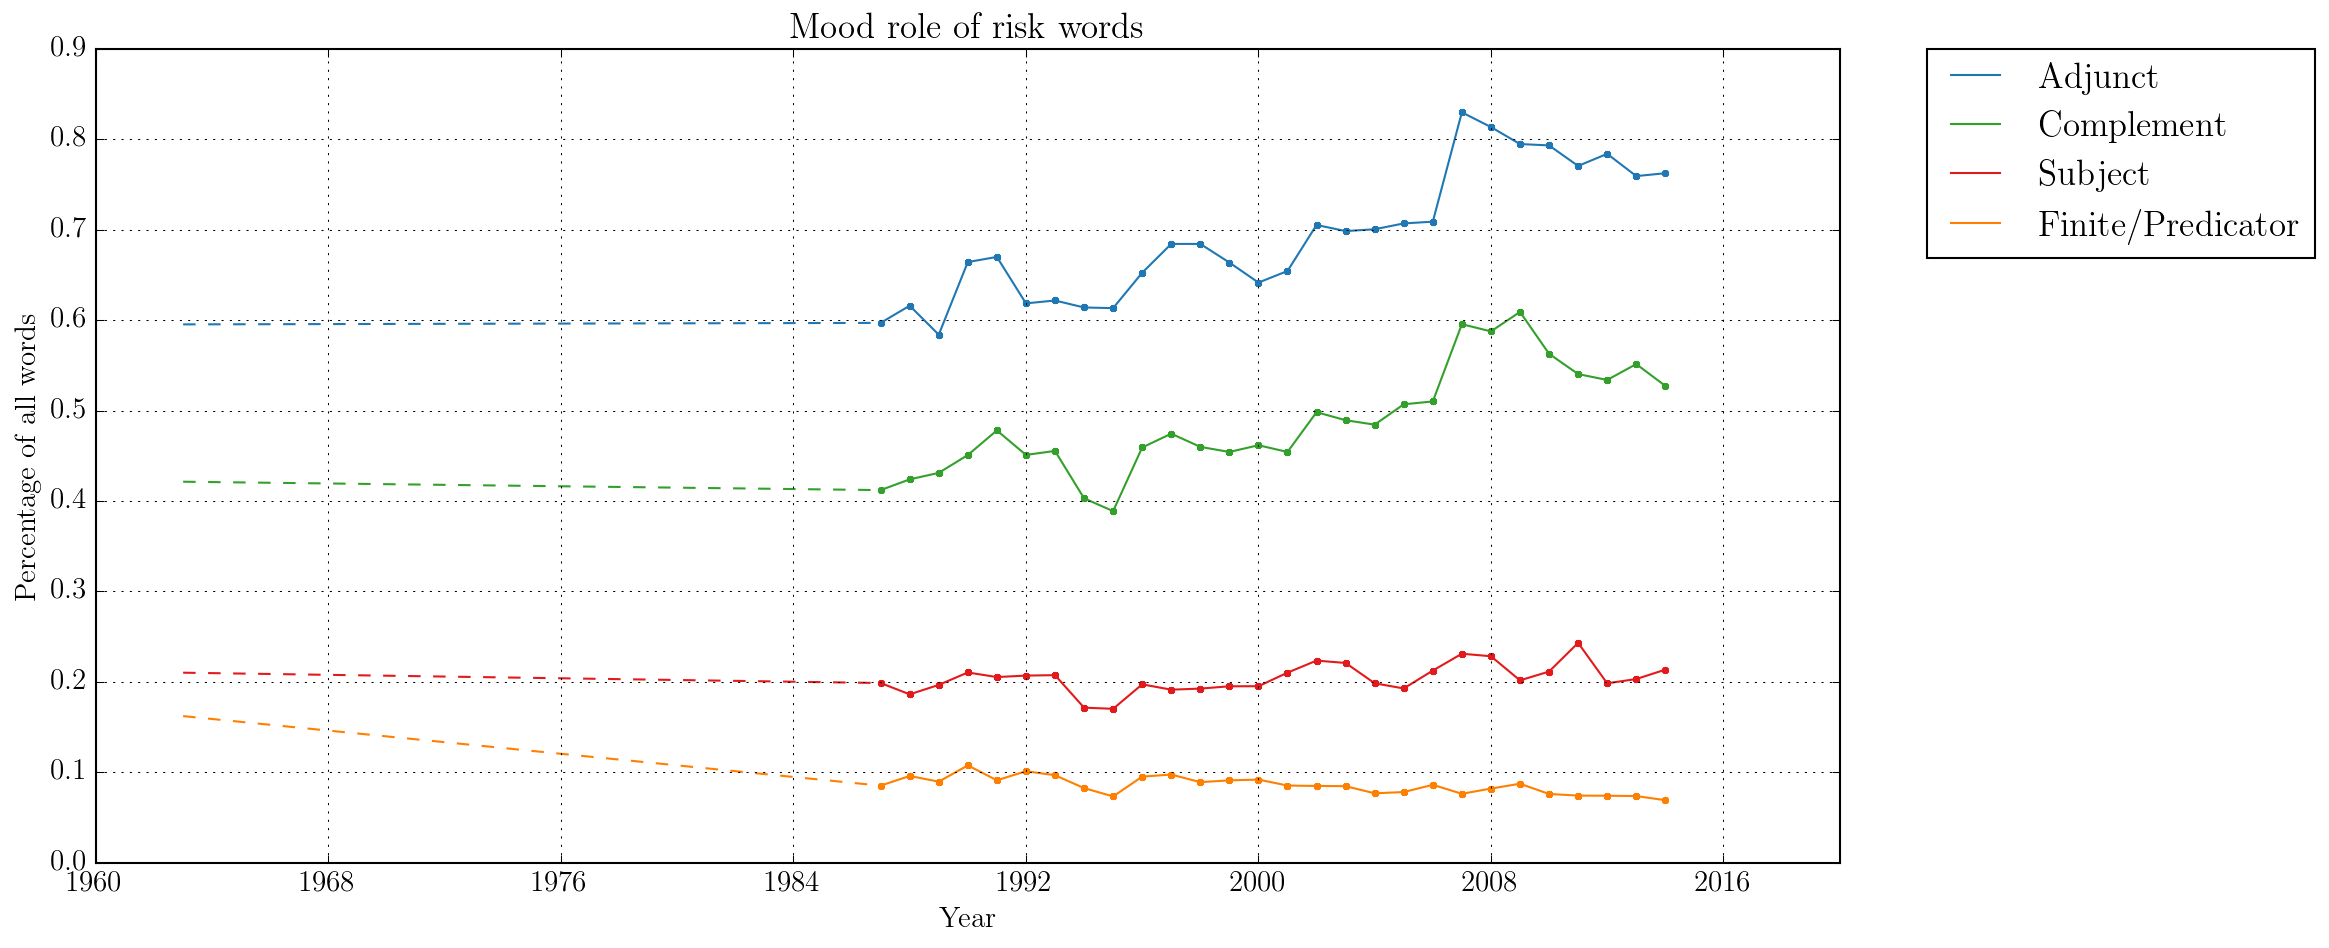
\includegraphics[width=0.98\textwidth]{../images/riskdep_allwords.png}
    \end{minipage}
    \caption{Frequency of risk words for each Mood component as percentage of all risk words\slash all parsed data}
    \label{fig:interpersonalarg}
    \end{figure}

    %By providing each role with a relative weight, we can plot arguability as a single decreasing trend line, showing the increased implicitness of risk within the language of the NYT.

    %Using the full list of risk dependencies, we can also locate more specific constructions undergoing trajectory shift. Figure \ref{fig:salienttrajectories} shows that risk is increasingly instantiated within prepositional phrases (which are by their nature dependent on Participants and Processes), and decreasingly as a predicator. From this view too, risk words are increasingly implicit within news language.

    \vspace{5mm}\noindent\begin{tcolorbox}[colback=yellow!5,colframe=yellow!40!black,title=Summary: risk and arguability]
    \parbox{1\textwidth}{%
    Longitudinally, risk words are shifting to less focal parts of clauses. We can approximate these changes using both indices or semantic function information within dependency parses.}
    \end{tcolorbox}
    \vspace{5mm}

\section{Risk words and proper nouns} \FloatBarrier

    We searched for proper noun groups in parse trees containing a risk word. This is a departure from many of our earlier queries, as here we are looking only at which entities co-occur with risk language, rather than determining how risk words and non-risk words relate to other another lexicogrammatically. The result of this query was 68891 different proper noun groups. We took the 200 most common results, and merged any that denoted the same entity: \emph{F.D.A.\slash Food and Drug Administration}, or \emph{Federal Reserve and Fed}. We then grouped results into thematic categories: \emph{People}, \emph{Nations}, \emph{Geopolitical entities}, \emph{Companies}, \emph{Organisations} and \emph{Medical themes}. The results were then plotted (See Figure \ref{fig:propernouns}). 

    \begin{landscape}
    \centering
    \begin{figure}
    \captionsetup[subfigure]{oneside,margin={-1.5cm,-.5cm}}
    \centering % [t!] % "[t!]" placement specifier just for this example
    \begin{subfigure}{.64\textwidth}
    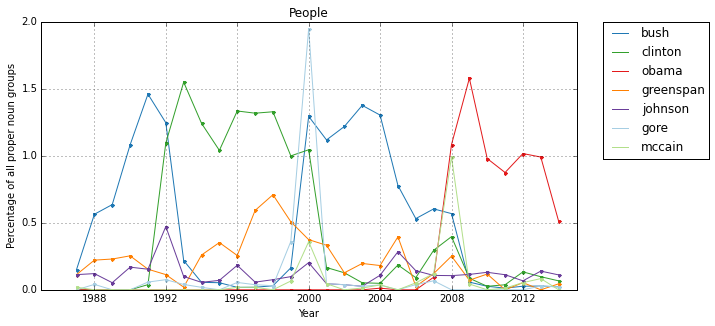
\includegraphics[width=\linewidth]{../images/people}
    \caption{People} \label{fig:a}
    \end{subfigure}
    \begin{subfigure}{.64\textwidth}
    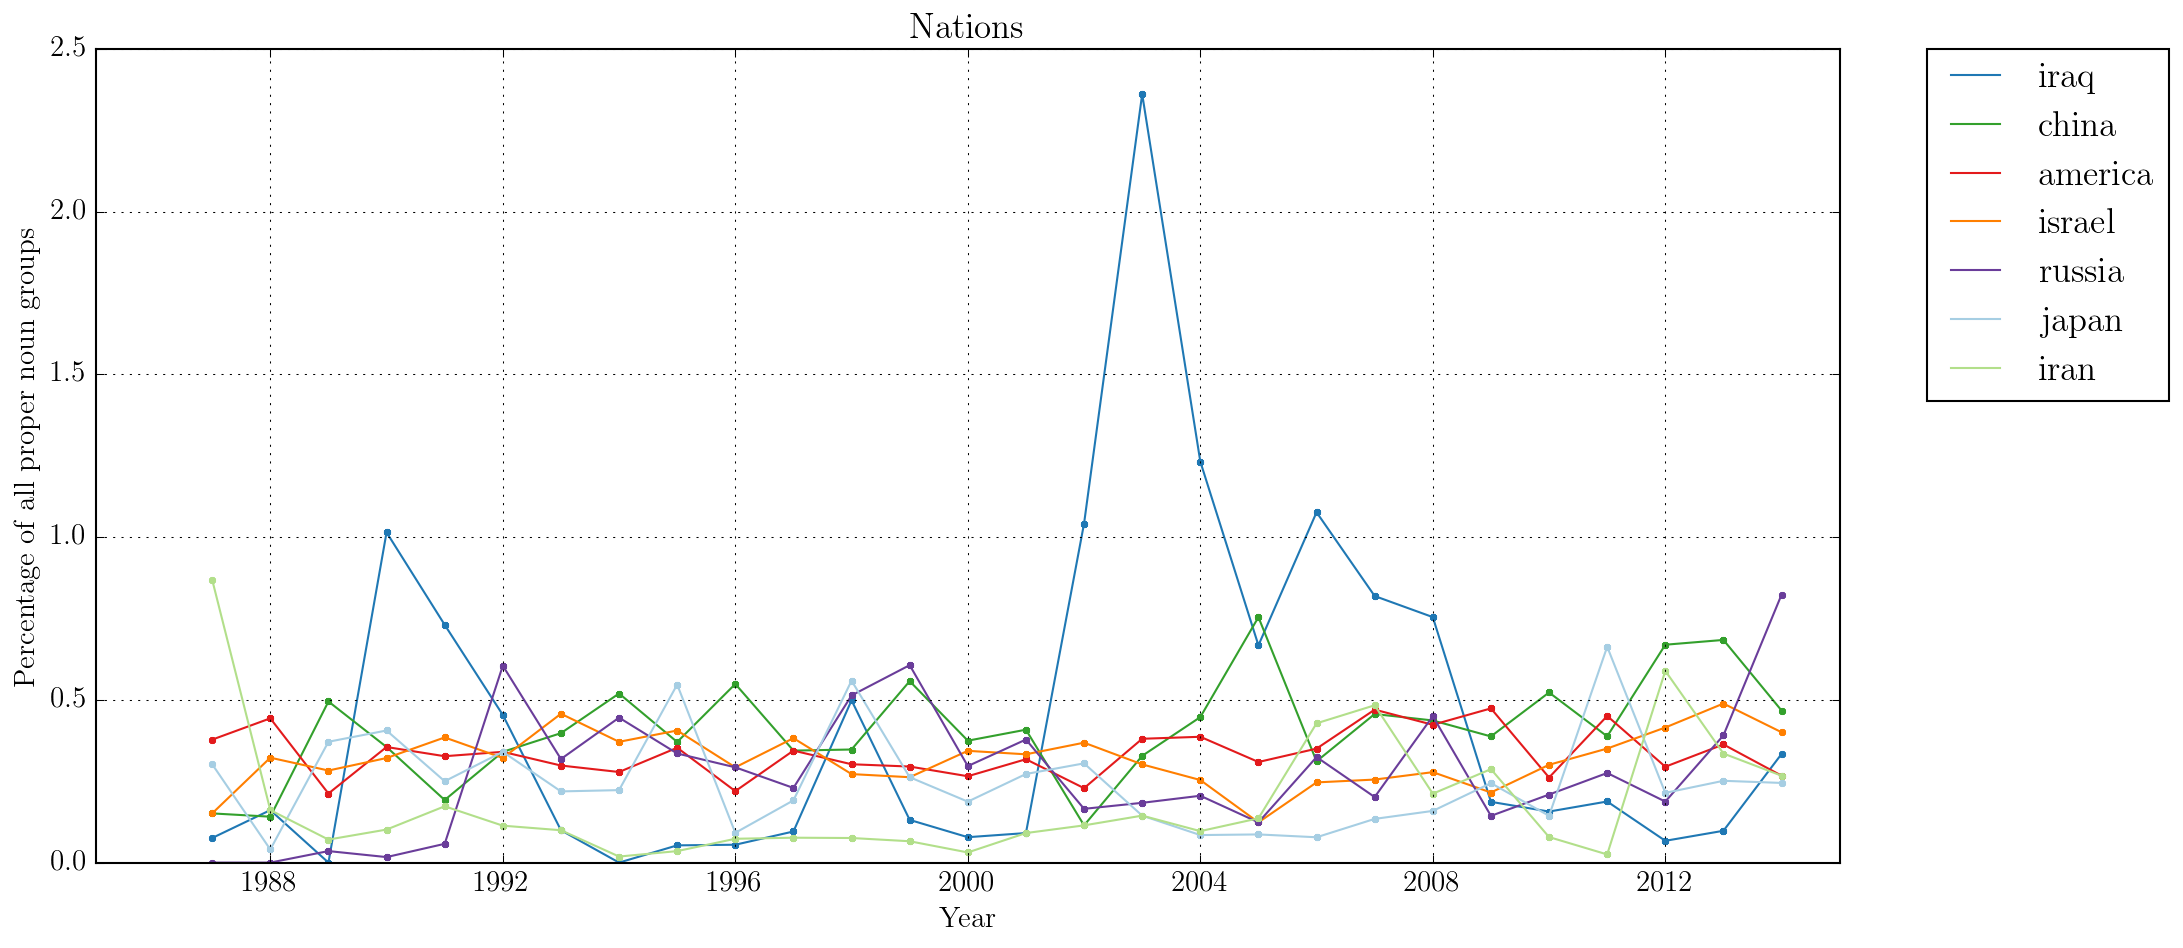
\includegraphics[width=\linewidth]{../images/nations}
    \caption{Nations} \label{fig:b}
    \end{subfigure}

    \medskip
    \begin{subfigure}{.64\textwidth}
    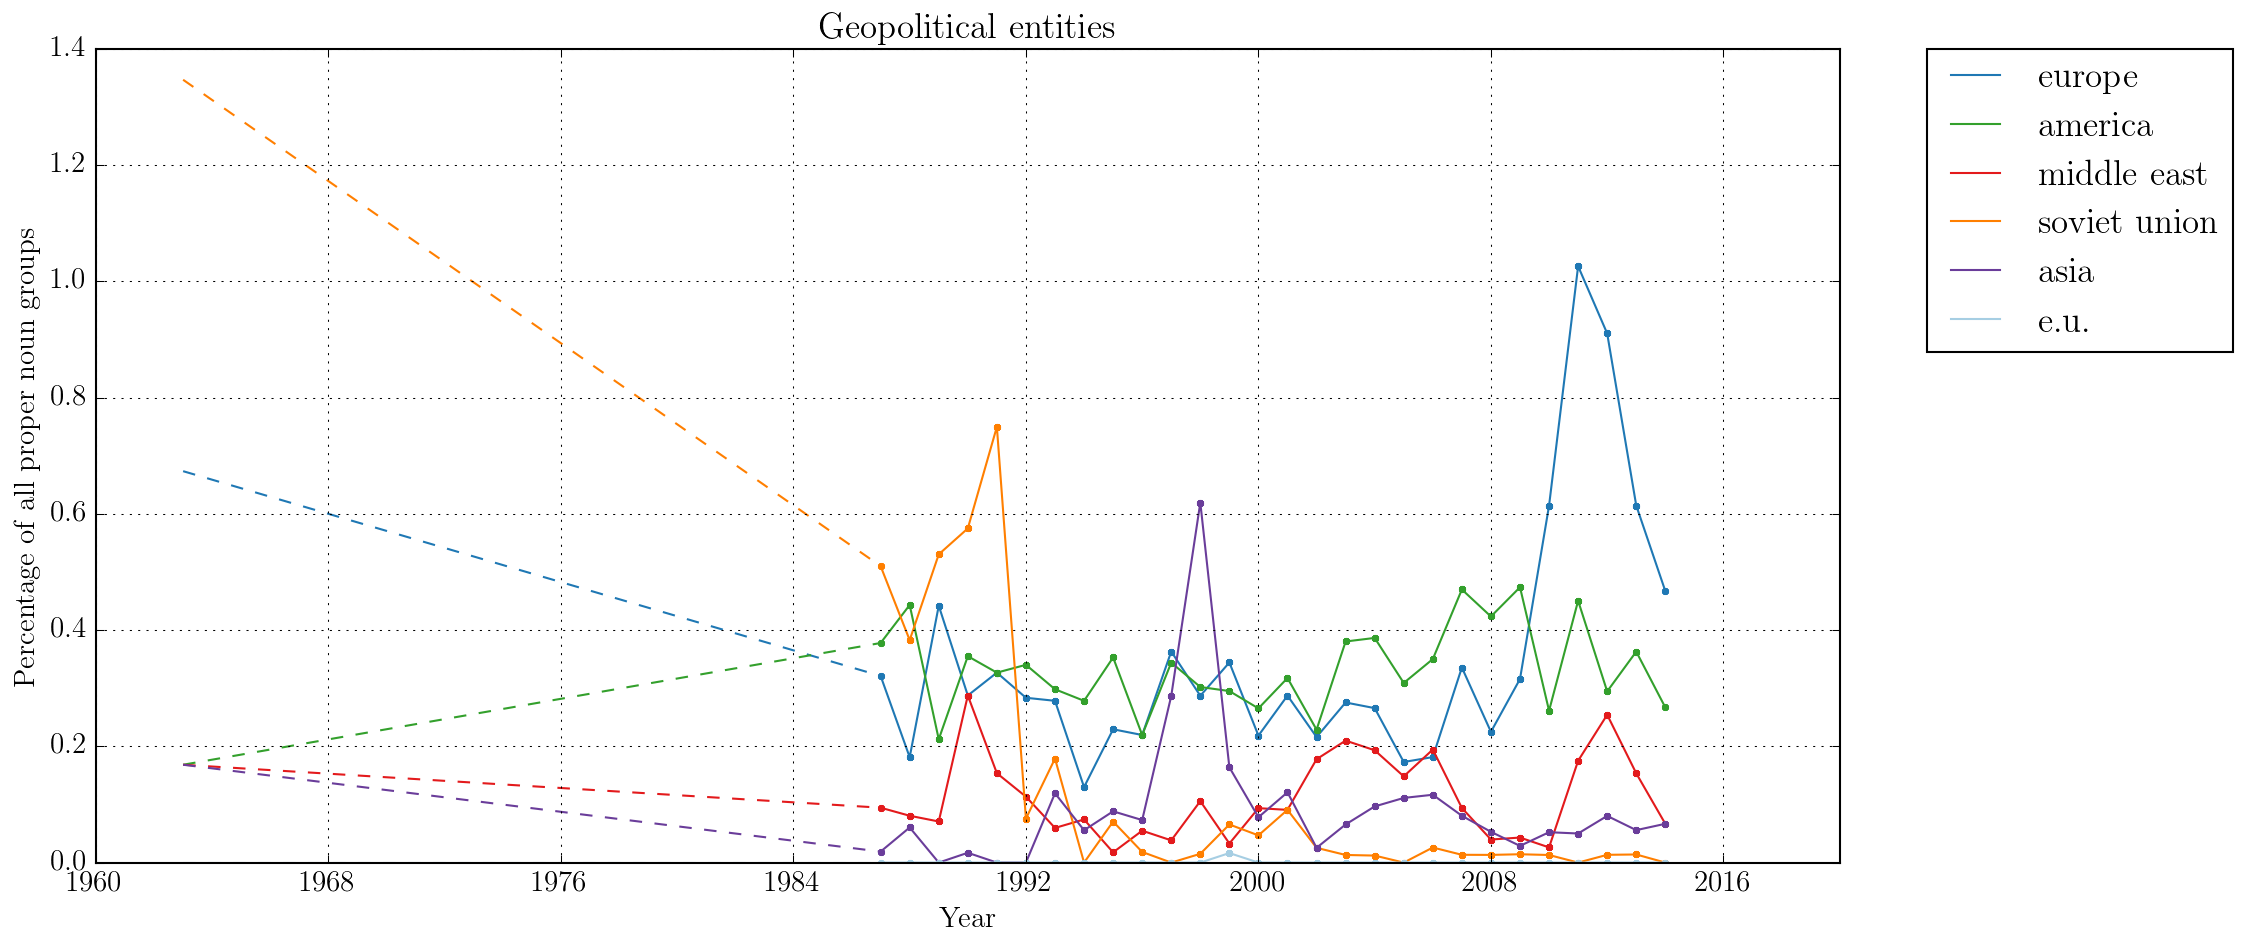
\includegraphics[width=\linewidth]{../images/geopolitical_entities}
    \caption{Geopolitical entities} \label{fig:c}
    \end{subfigure}
    \begin{subfigure}{.64\textwidth}
    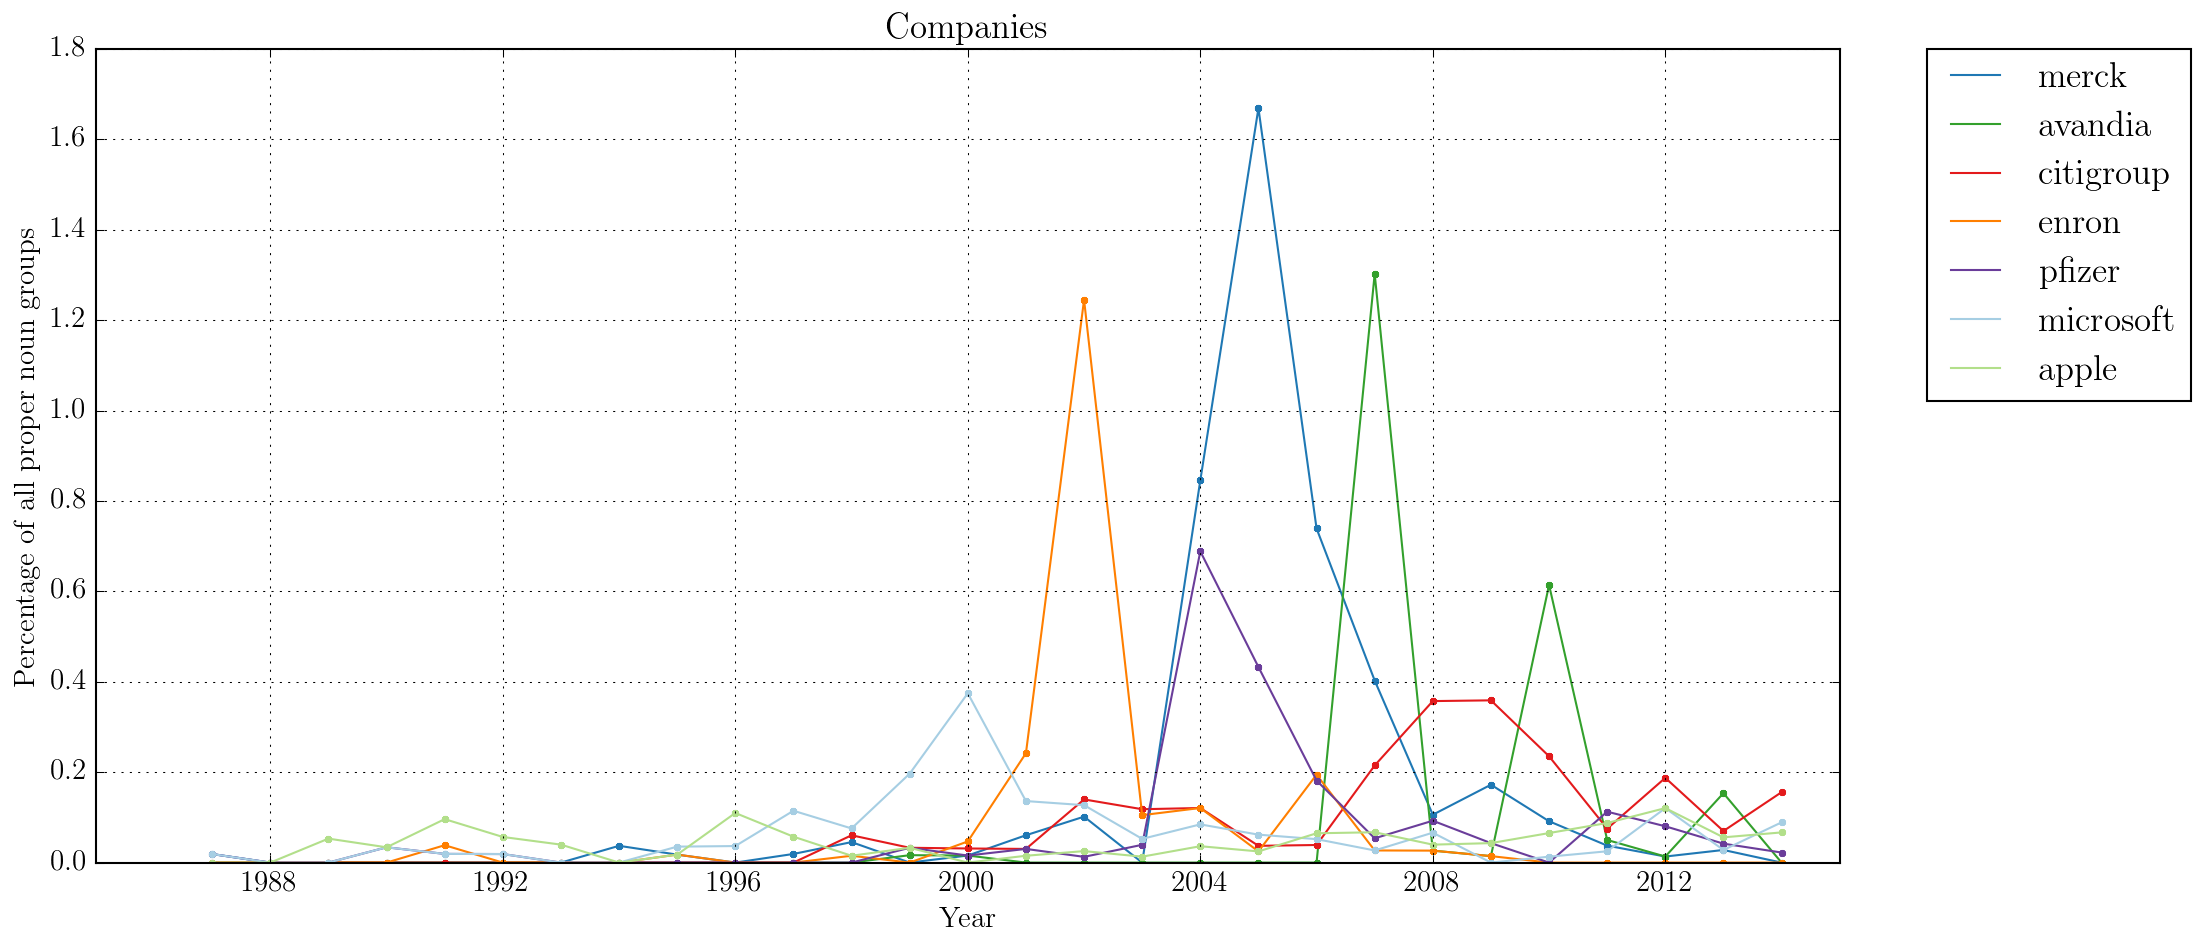
\includegraphics[width=\linewidth]{../images/companies}
    \caption{Companies} \label{fig:d}
    \end{subfigure}

    \medskip
    \begin{subfigure}{.64\textwidth}
    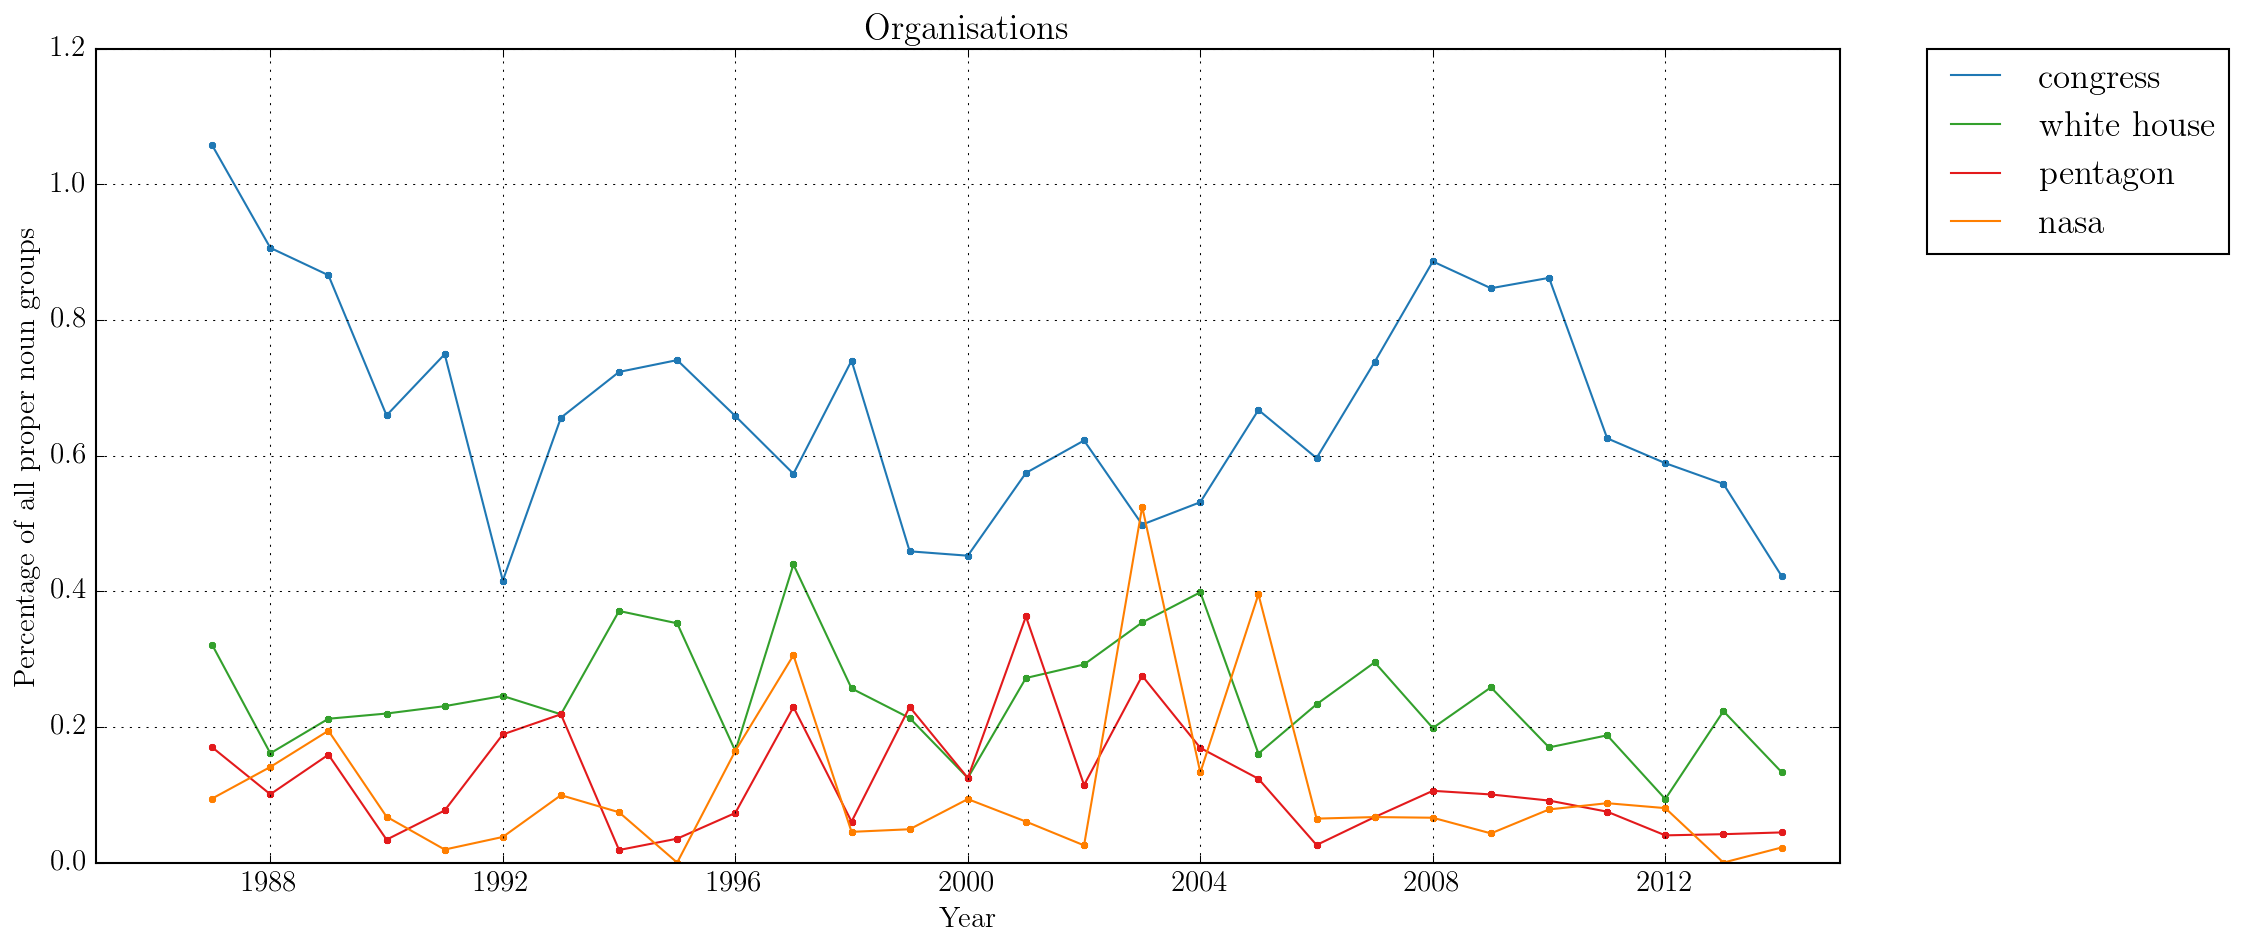
\includegraphics[width=\linewidth]{../images/organisations}
    \caption{Organisations} \label{fig:e}
    \end{subfigure}
    \begin{subfigure}{.64\textwidth}
    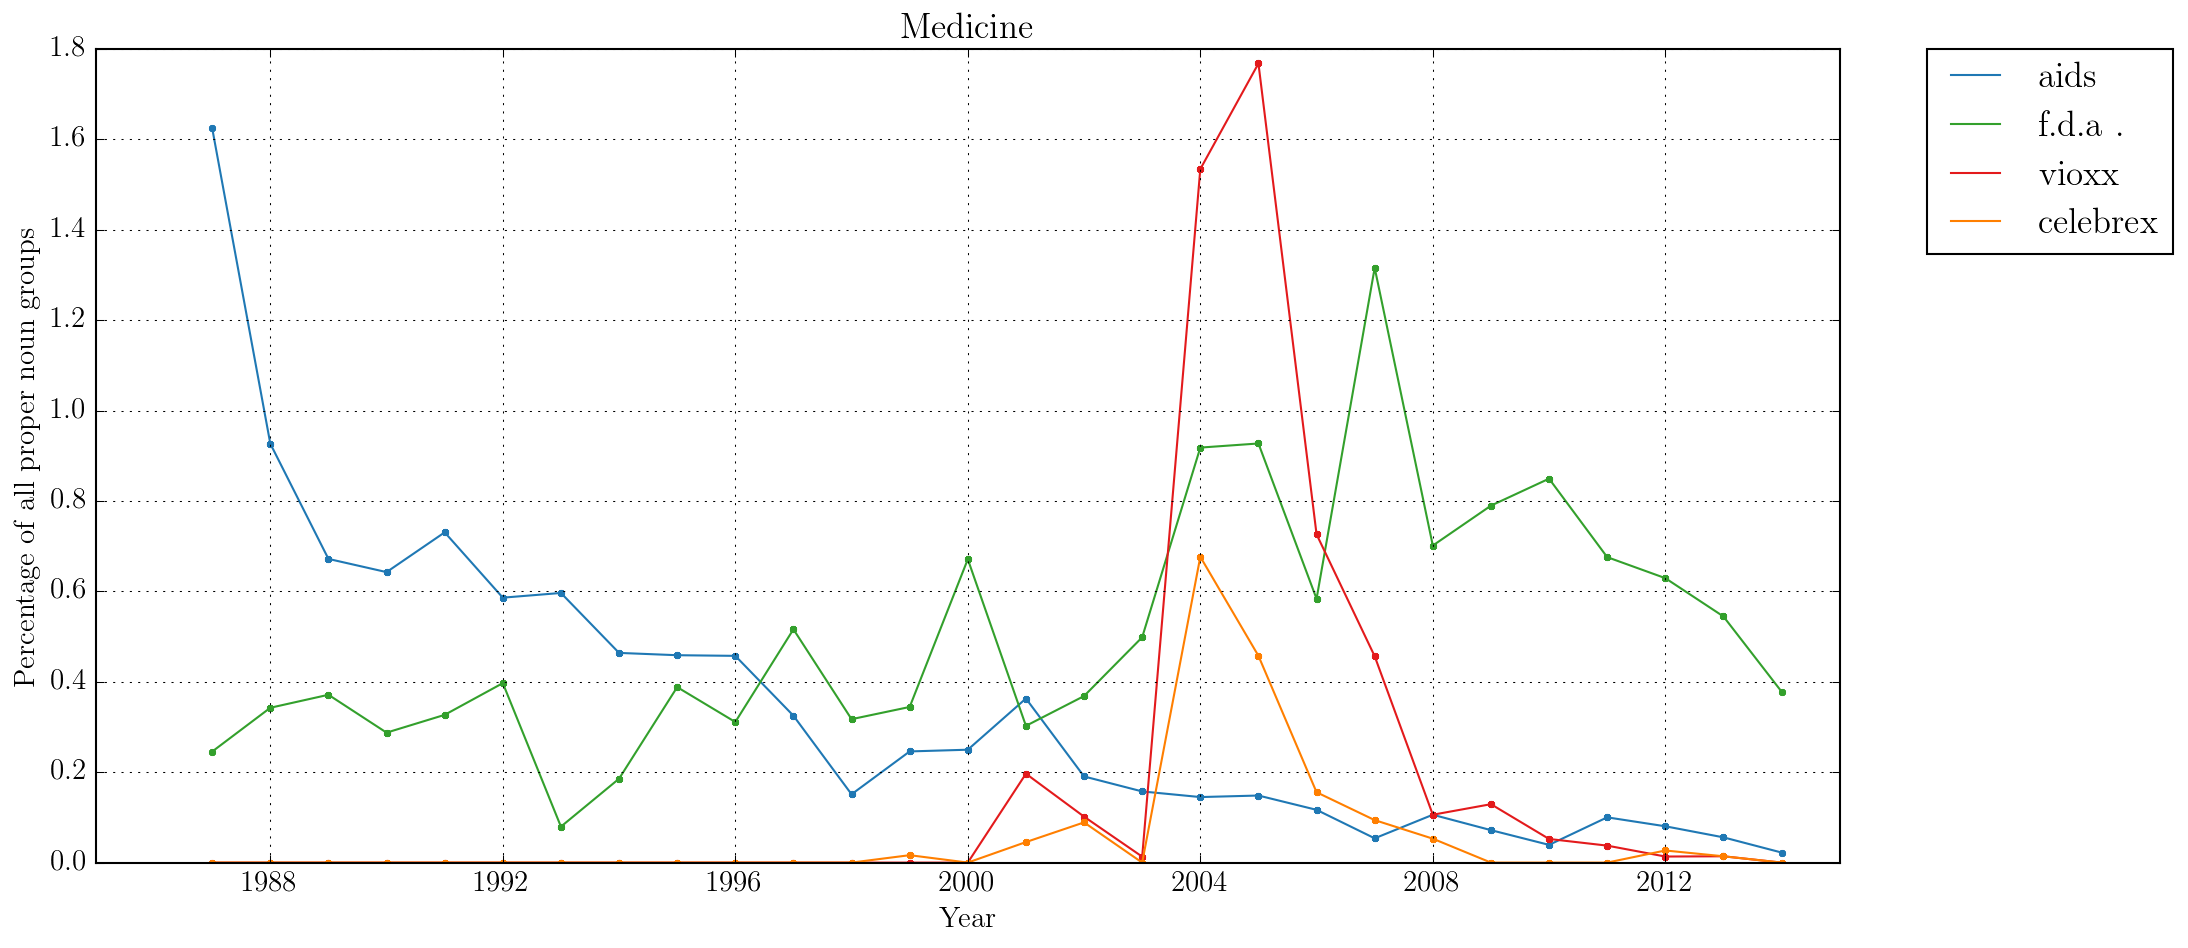
\includegraphics[width=\linewidth]{../images/medicine}
    \caption{Medical terms} \label{fig:f}
    \end{subfigure}
    \caption{Proper noun groups co-occurring with risk} \label{fig:propernouns}
    \end{figure}
    \end{landscape}

    A number of historical events were easily recognisable within the peaks and troughs of these charts. Key events represented through these interrogations include:

    \begin{enumerate} \setlength\itemsep{0em}
    \item US presidents and presidential candidates\endnote{Though the filtering out of titles and given names collapses the distinction between Bushes and Clintons, we can still reasonably infer which was being spoken about at which, and doubt can be eliminated by concordancing}~(Figure~\ref{fig:a})
    \item The First Persian Gulf War (Figure~\ref{fig:b})                   
    \item The Iraq Wars (Figure~\ref{fig:b})
    \item September 11 and the War in Afghanistan (Figure~\ref{fig:b})   
    \item The beginning of the 2014 Crimean crisis (Figure~\ref{fig:b})       
    \item The Asian financial crisis (Figure~\ref{fig:c})
    \item The breakup of the Soviet Union (Figure~\ref{fig:c})
    \item The Eurozone crisis (Figure~\ref{fig:c})
    \item The Space Shuttle Colombia Disaster (Figure~\ref{fig:d})
    \item The collapse of Enron (Figure~\ref{fig:e})
    \item The U.S. subprime mortgage crisis  (Figure~\ref{fig:e})
    \item The U.S. outbreak of HIV and the AIDS crisis (Figure~\ref{fig:f})
    \item The recall of Vioxx (Figure~\ref{fig:f})
    \end{enumerate}
    %
    This area of our investigation is by far the most promising as a means of connecting risk language to particular people and events. Spatial considerations have precluded a full treatment of the charting of risk language to specific events, despite the fact that enough data exists for detailed analyses of any number of potential foci. Future research that centres on detailed exploration of health domains (including the Vioxx recall) is planned.

    \vspace{5mm}\noindent\begin{tcolorbox}[colback=yellow!5,colframe=yellow!40!black,title=Summary: risk and proper nouns]
    \parbox{1\textwidth}{%
    We can use proper nouns to see which people, places and things co-occur with discussion of risk.}
    \end{tcolorbox}
    \vspace{5mm}

\section{Summary of key findings}

    We found that the behaviour of risk words has changed longitudinally in a number of key respects:

    \begin{enumerate}
    \item Risk words appear to be increasing in relative frequency, with modest increases in the number of unique risk words per year.
    \item Risk as a process is declining in use, and has been overtaken in frequency by risk as a participant.
    \item Risk is more often an experiential object than an experiential subject. The gap has widened considerably over time.
    \item \emph{Calculated risk} has been overtaken by \emph{potential risk} in overall frequency. \emph{High-risk} spikes in frequency in references to H5N1.
    \item When risk is a participant, quantification is often at the centre of the experiential meaning. The high proportion of mental processes highlights a portrayal of risks as perceived.
    \item Both \emph{pose risk} and \emph{put at risk} have overtaken \emph{run risk} in frequency. Use of the prototypical risk process, \emph{to risk} is declining. Finally, there is some evidence for reduced agency the \emph{run risk} process.
    \item When risk is a process, risked things\slash potential harms often pertain to individual health. This contrasts with processes as potential harm, which generally relate to people in positions of power.
    \item Common risk modifiers (\emph{risky}, \emph{riskier}, \emph{riskiest}) are gradually being displaced by a number of less common constructions (e.g. \emph{low-risk}, \emph{at-risk}, \emph{risk-averse}, \emph{risk-free})
    \item While risk as a modifier is often used in the context of finance\slash commerce, \emph{at-risk} typically attaches to vulnerable human demographics.
    \item  Longitudinally, risk words are shifting to less focal parts of clauses. We can approximate these changes using both indices or semantic function information within dependency parses.
    \item Proper nouns co-occurring with risk words highlight the close relationship between risk and health discourse.
    \end{enumerate}
    %
    As will be discussed in Chapter \ref{chap:discussion}, many of these shifts appear to be a part of a broader discourse-semantic trend of implicitness and inarguability of risk. 

    % In the following chapter, interrogations used here are applied to subcorpora of Economics, Politics and Health articles.

